% =====================================================================
%   Tesis: Traduccion automatica neuronal Shiwilu - Castellano
%   Autor:   Fabian Prado Infanson
%   Asesor:  Hector Gomez
%   Convertido desde Word (.docx) con Pandoc + limpieza manual
%   Compilar con (para resolver citas y referencias APA):
%       xelatex tesis.tex
%       biber   tesis
%       xelatex tesis.tex
%       xelatex tesis.tex
%   o, si tienes latexmk:  latexmk -xelatex tesis.tex
% =====================================================================

\documentclass[12pt,a4paper,oneside]{book}

% --- Codificacion e idioma (xelatex) ---
\usepackage{fontspec}
\usepackage{polyglossia}
\setmainlanguage{spanish}

% --- Geometria, espaciado y tipografia (perfil cercano a APA 7, trabajo estudiantil) ---
% A4; margenes 1" (~2,54 cm) en todos los lados (APA 7).
% nohead: no reserva espacio para cabeceras corrientes (libera ~37 pt encima del cuerpo).
\usepackage[a4paper,margin=1in,nohead]{geometry}
\usepackage{setspace}
\doublespacing
\usepackage{microtype}
% Estilo bloque: sin sangria de primera linea; los parrafos se separan por un
% pequeno espacio vertical. Evita el efecto de "la primera linea queda corrida
% respecto al resto del parrafo" presente al usar sangria APA tradicional.
\setlength{\parindent}{0pt}
\setlength{\parskip}{6pt plus 1pt minus 0pt}
% Times New Roman 12 pt (clase ya pide 12pt). Si falla la fuente, usar p. ej. TeX Gyre Termes.
\setmainfont{Times New Roman}[
  Ligatures = {Common, TeX},
]
\usepackage{etoolbox}
% titlesec redefine \chapter pero NO siempre toca \@makeschapterhead (la macro
% que book.cls usa internamente para \chapter*). Por eso parchamos los vskip de
% book.cls aqui: aunque titlesec controle el "outer spacing", el "inner spacing"
% sigue viniendo de book.cls. Sin estos parches \chapter* (Resumen, Referencias)
% queda con ~90 pt de blanco fantasma encima.
\makeatletter
\patchcmd{\@makechapterhead}{\vspace*{50\p@}}{\vspace*{0pt}}{}{}
\patchcmd{\@makechapterhead}{\vskip 20\p@}{\vskip 6\p@}{}{}
\patchcmd{\@makechapterhead}{\vskip 40\p@}{\vskip 12\p@}{}{}
\patchcmd{\@makeschapterhead}{\vspace*{50\p@}}{\vspace*{0pt}}{}{}
\patchcmd{\@makeschapterhead}{\vskip 40\p@}{\vskip 12\p@}{}{}
\makeatother

% Espaciado compacto para \chapter, \section, \subsection, \subsubsection y \paragraph.
% titlesec da control fino sin tener que redefinir \@startsection a mano.
\usepackage{titlesec}
% Chapter: formato bloque (numero "Capitulo N" en linea separada arriba del titulo,
% Huge negrita) y espacio MUY reducido arriba (0pt) y debajo (1ex).
\titleformat{\chapter}[display]
  {\normalfont\Huge\bfseries\raggedright}
  {\huge\bfseries\chaptertitlename\ \thechapter}
  {6pt}
  {}
% Para \chapter* (Resumen, Referencias) usamos shape [block]: sin label vacio
% que genere una linea fantasma de \Huge \baselineskip (~52 pt con doublespacing).
\titleformat{name=\chapter,numberless}[block]
  {\normalfont\Huge\bfseries\raggedright}
  {}
  {0pt}
  {}
% Espaciado antes/despues del titulo de capitulo. Hay que declarar las DOS
% variantes: titlesec NO hereda automaticamente el spacing de la version
% numerada al chapter*.
\titlespacing*{\chapter}                       {0pt}{0pt}{1.2ex}
\titlespacing*{name=\chapter,numberless}       {0pt}{0pt}{1.2ex}
\titlespacing*{\section}      {0pt}{1.2ex plus 0.4ex minus 0.2ex}{0.8ex plus 0.2ex}
\titlespacing*{\subsection}   {0pt}{1.0ex plus 0.3ex minus 0.2ex}{0.6ex plus 0.2ex}
\titlespacing*{\subsubsection}{0pt}{0.8ex plus 0.2ex minus 0.2ex}{0.4ex plus 0.2ex}
\titlespacing*{\paragraph}    {0pt}{0.6ex plus 0.2ex minus 0.1ex}{0.5em}
% Tablas largas: espacio sencillo dentro de la tabla; fuera se mantiene doble.
\AtBeginEnvironment{longtable}{\singlespacing}
\AfterEndEnvironment{longtable}{\doublespacing}

% --- Graficos / imagenes ---
\usepackage{graphicx}
\graphicspath{{figuras/}{figuras/media/}}

% --- Colores ---
\usepackage{xcolor}

% --- Tablas (longtable, multipagina; estilo APA: sin verticales, booktabs) ---
\usepackage{longtable}
\usepackage{booktabs}
\usepackage{array}
\usepackage{calc}
\usepackage{multirow}
\usepackage{caption}
\captionsetup[table]{name=Tabla}
\captionsetup[longtable]{
  labelfont=bf,
  textfont=normalfont,
  position=top,
  skip=6pt,
}
\renewcommand{\arraystretch}{1.25}

% --- Matematicas ---
\usepackage{amsmath}
\usepackage{amssymb}
\usepackage{amsfonts}

% --- Listas mejoradas ---
\usepackage{enumitem}

% --- Citas, hipervinculos y referencias cruzadas ---
\usepackage[colorlinks=true,
            linkcolor=blue!50!black,
            citecolor=blue!50!black,
            urlcolor=blue!50!black,
            bookmarksnumbered=true]{hyperref}

% --- Bibliografia APA 7 con biblatex + biber ---
% Cargado despues de polyglossia/hyperref para que la localizacion
% castellana de las cadenas APA (y, et al., pp., etc.) tome efecto.
\usepackage[backend=biber,
            style=apa,
            sortlocale=es_ES,
            sorting=nyt,
            language=spanish]{biblatex}
\DeclareLanguageMapping{spanish}{spanish-apa}
\addbibresource{tesis.bib}
% Sangria francesa de la bibliografia: por defecto biblatex usa ~0.5",
% que contrasta mucho con el cuerpo en estilo bloque. Se reduce a 0.25"
% (compromiso visual entre legibilidad y coherencia con el resto del documento).
\setlength{\bibhang}{0.25in}

% --- Resaltado (\hl) usado por Pandoc ---
\usepackage{soul}

% --- Comandos auxiliares que Pandoc puede emitir ---
\providecommand{\tightlist}{%
  \setlength{\itemsep}{0pt}\setlength{\parskip}{0pt}}
\providecommand{\real}[1]{#1}
\providecommand{\pandocbounded}[1]{#1}

% --- Metadatos del PDF ---
\hypersetup{
  pdftitle={Traduccion automatica neuronal Shiwilu - Castellano},
  pdfauthor={Fabian Prado Infanson},
  pdfsubject={Tesis - Ingenieria Informatica - PUCP},
  pdfkeywords={NMT, Shiwilu, Castellano, lenguas de bajo recurso, traduccion automatica neuronal}
}

% =====================================================================
\begin{document}
\pagestyle{plain}

% Sin numeracion de capitulos en la caratula y resumen (frontmatter)
% Los \chapter dentro de tesis_raw.tex usan la numeracion arabiga normal.

% =====================================================================
%  CARÁTULA
% =====================================================================
\begin{titlepage}
  \centering
  \vspace*{1cm}

  {\large\textbf{PONTIFICIA UNIVERSIDAD CATÓLICA DEL PERÚ}}\\[0.3cm]
  {\large\textbf{FACULTAD DE CIENCIAS E INGENIERÍA}}\\[1.5cm]

  
\includegraphics[width=5cm]{media/image1.png}\\[1.5cm]

  {\Large\textbf{``Traducción automática neuronal Shiwilu--Castellano''}}\\[0.8cm]

  {\large\textbf{Tesis para obtener el título profesional de Ingeniería Informática}}\\[2cm]

  \textbf{AUTOR:}\\[0.2cm]
  Fabian Prado Infanson\\[1cm]

  \textbf{ASESOR:}\\[0.2cm]
  Hector Gómez\\[2cm]

  {\large Lima, 26 de Julio del 2025}
\end{titlepage}

% =====================================================================
%  RESUMEN
% =====================================================================
\chapter*{Resumen}
\addcontentsline{toc}{chapter}{Resumen}


\clearpage
\tableofcontents
\clearpage
\listoftables
\clearpage

\chapter{Generalidades}\label{generalidades}

\section{Problemática}\label{problemuxe1tica}

El shiwilu, también llamado jebero, es una lengua amazónica peruana de la familia cahuapana que atraviesa un estado crítico de amenaza. El número de hablantes es muy reducido, en su mayoría personas adultas mayores, y la transmisión intergeneracional se encuentra quebrada \parencite{valenzuela2018}. Aunque en 2016 fue declarada Patrimonio Cultural de la Nación, su presencia en el ecosistema digital sigue siendo mínima, lo que incrementa el riesgo de desplazamiento. Cuando una lengua no encuentra espacios de uso en entornos digitales, su marginación se acelera y disminuye la posibilidad de su aprendizaje y uso cotidiano \parencite{ministeriodecultura2016,unesco2023}.

En este escenario, un sistema de traducción automática neuronal entre shiwilu y castellano podría convertirse en una herramienta estratégica para documentar, acceder y circular conocimiento bilingüe. No obstante, el desarrollo de un traductor de este tipo enfrenta un cuello de botella inmediato: no existe un corpus paralelo shiwilu--castellano con volumen y diversidad suficientes para entrenar y evaluar modelos con criterios reproducibles. La traducción automática, tanto en su vertiente estadística como neuronal, depende de colecciones amplias de oraciones alineadas; cuando el paralelo es mínimo, la calidad de los modelos cae y los resultados no son comparables entre estudios \parencite{mager2018}. En shiwilu, más allá de aportes de documentación, como el diccionario bilingüe con ejemplos de uso, los datos disponibles siguen siendo escasos y dispersos, de modo que no hay baselines ni conjuntos de prueba estables contra los cuales contrastar avances \parencite{valenzuela2018}. Esta situación contrasta con pares mejor documentados en la región, como quechua--español o shipibo--español, donde ya existen corpus iniciales y evaluaciones básicas que permiten organizar la investigación \parencite{galarreta2017,chuquimamani2021}.

El problema abarca también la calidad y la representatividad de los datos. En ausencia de textos variados, el material disponible tiende a concentrarse en narrativas tradicionales o léxico especializado, lo que sesga el dominio temático y deja fuera construcciones frecuentes del uso cotidiano. Con pocos ejemplos, los modelos neuronales sobreajustan y generalizan mal, fenómeno documentado en lenguas indígenas con corpus de apenas miles de oraciones \parencite{mager2018}. A ello se suma la distancia tipológica entre shiwilu y castellano: la morfología aglutinante, ciertos patrones estructurales y los alineamientos semánticos no uno a uno complica la alineación y la traducción literal de términos culturalmente marcados; en varios casos no hay equivalencias directas, lo que exige una curación cuidadosa y verificación contextual de las parejas de oración \parencite{ministeriodecultura2016}. Incluso si se reúne un primer conjunto paralelo, la calidad del dato y su adecuación semántica y cultural se vuelven el desafío central.

La dimensión sociolingüística es igualmente ineludible, ya que la construcción de recursos depende del trabajo con hablantes. Dada la escala de la comunidad y la edad de sus miembros, la obtención y validación de paralelos requiere colaboración cercana. En este proyecto, el Grupo Chana ha articulado la recolección de materiales con apoyo del señor Fidel Lomas Chota, hablante competente y autor de relatos en shiwilu, quien ha contribuido con traducciones y validaciones. Su participación garantiza datos de primera mano y criterio cultural para juzgar la aceptabilidad de equivalencias, un aspecto que las métricas automáticas no capturan por sí solas \parencite{unesco2023}. La experiencia comparada en náhuatl y guaraní sugiere, además, que sin esta mediación humana los modelos tienden a aprender artefactos del corpus y fallan en variedades o géneros no cubiertos por los datos de entrenamiento \parencite{rios2019,baladon2024}.

El panorama regional confirma que la base del problema en lenguas de muy bajos recursos es doble: escasez de corpus y ausencia de referencias evaluativas. En quechua sureño, la creación de nuevos conjuntos bilingües a partir de fuentes dispersas fue condición previa para evaluar con métricas estándar y establecer comparaciones significativas; sin ese piso de datos, no era posible justificar avances ni orientar mejoras \parencite{chuquimamani2021}. En shipibo--español, un esfuerzo temprano desde el enfoque estadístico mostró el mismo patrón: antes de buscar la mejor arquitectura, era imprescindible contar con un corpus alineado utilizable y un procedimiento reproducible para entrenar y medir \parencite{galarreta2017}. Estas lecciones sugieren que, en shiwilu, no hay atajos de ingeniería: sin un primer corpus paralelo confiable y criterios de evaluación claros, cualquier intento de traducción neuronal carecerá de base metodológica y relevancia práctica \parencite{meque2023}.

En síntesis, la problemática que aborda esta tesis es multidimensional. En el plano técnico, falta el insumo esencial, el cual es un corpus paralelo validado y por arrastre, faltan líneas de base y protocolos de evaluación adaptados al par shiwilu--castellano. En el plano lingüístico, la asimetría tipológica y la carga cultural de numerosos términos exigen datos cuidadosamente curados y verificación contextual. En el plano social, la escala pequeña y envejecida de la comunidad obliga a que la construcción de recursos sea participativa, pues solo así se asegura que las traducciones sean útiles y respetuosas \parencite{unesco2023}. Mantener este conjunto de factores sin atender mantiene al shiwilu fuera del ecosistema digital y limita su aprendizaje, su circulación escrita y su presencia simbólica en la esfera pública.

Este diagnóstico delimita con precisión el núcleo del problema: sin corpus paralelo validado, sin líneas de base y sin un esquema de verificación que combine métricas automáticas con revisión por hablantes, no es posible avanzar con rigor hacia un traductor neuronal shiwilu$\leftrightarrow$castellano. Por ello, esta investigación asume como punto de partida la construcción y depuración de datos bilingües con apoyo comunitario, junto con la definición de criterios evaluativos reproducibles que permitan situar cualquier resultado en una línea cero clara. Solo sobre ese cimiento será razonable explorar y comparar arquitecturas, estrategias de transferencia y futuros incrementos de datos. Atender esta problemática no solo llena un vacío científico en la traducción automática de lenguas peruanas de muy bajo recurso; también supone un paso concreto para que el shiwilu tenga presencia en la esfera tecnológica contemporánea \parencite{valenzuela2018,unesco2023}.

\subsection{Árbol de Problemas}\label{uxe1rbol-de-problemas}

En la figura 1 se muestra un panorama claro para observar la problemática central, las causas consideradas y consecuencias que generan estas mismas.

\begin{figure}[h]
\centering
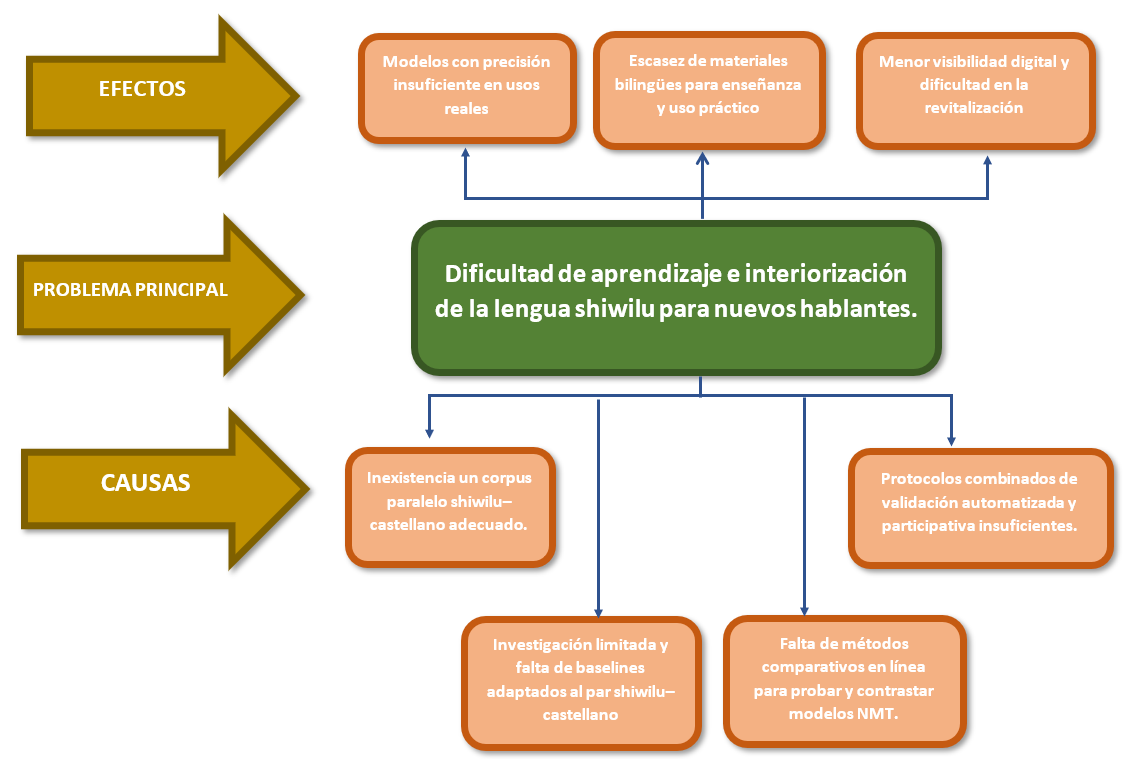
\includegraphics[width=\linewidth,alt={Árbol de problemas del proyecto}]{media/image2.png}
\caption{Árbol de Problemas}
\label{fig:arbol-problemas}
\end{figure}

\subsection{Causas}\label{causas}

\paragraph{Inexistencia de un corpus paralelo shiwilu--castellano adecuado.}
Los textos disponibles son escasos, dispersos y con variaciones ortográficas y de dominio que dificultan su aprovechamiento. Falta alineación fiable a nivel de oración, hay ruido (traducciones parciales, glosas, duplicados) y metadatos incompletos. Además, no existen particiones estandarizadas de entrenamiento/validación/prueba que permitan comparaciones justas y reproducibles.

\paragraph{Investigación limitada y falta de baselines adaptados al par shiwilu--castellano.}
Hay pocos estudios específicos y no se cuenta con líneas base consensuadas (configuraciones mínimas, tokenización/segmentación apropiada o variantes multilingües razonables). Esta carencia impide medir avances con rigor, aislar el impacto de cada técnica y evitar conclusiones sesgadas por configuraciones ad-hoc.

\paragraph{Falta de métodos comparativos en línea para probar y contrastar modelos NMT.}
No existe una interfaz accesible que permita evaluar modelos lado a lado, registrar métricas y recopilar ejemplos de uso real de forma ágil. Sin pruebas comparativas en un entorno web, se ralentiza el ciclo de retroalimentación, se dificulta la trazabilidad de cambios y se limita la participación de docentes e integrantes de la comunidad.

\paragraph{Protocolos combinados de validación automatizada y participativa insuficientes.}
Predomina el uso de métricas automáticas generales que no capturan adecuación, naturalidad ni pertinencia cultural. Faltan guías, instrumentos y criterios para integrar la revisión de hablantes (escalas, rúbricas, taxonomías de error, control de acuerdo inter-anotador), lo que genera evaluaciones incompletas y poco accionables.

\subsection{Consecuencias}\label{consecuencias}

\paragraph{Modelos con precisión insuficiente en usos reales.}
Las salidas presentan errores léxicos y morfosintácticos, inestabilidad ante variantes ortográficas y pérdida de sentido en dominios no vistos. Esto reduce la confianza de usuarios y docentes, eleva el costo de posedición y limita la adopción del traductor en tareas cotidianas (material educativo, comunicaciones comunitarias, trámites), dejando el sistema como un prototipo poco útil fuera del laboratorio.

\paragraph{Escasez de materiales bilingües para enseñanza y uso práctico.}
La falta de recursos paralelos limpios y actualizados impide generar textos, ejercicios y guías bilingües con progresión pedagógica. Se restringen las oportunidades de lectura y escritura en shiwilu con apoyo del castellano, y se dificulta producir contenidos para contextos reales (salud, servicios públicos, señalética), perpetuando la dependencia de materiales aislados o desactualizados.

\paragraph{Menor visibilidad digital y dificultad en la revitalización.}
La baja disponibilidad de herramientas y contenidos en línea reduce la presencia del shiwilu en buscadores, plataformas y aplicaciones, desincentivando la participación de jóvenes y hablantes potenciales. Esto crea un círculo vicioso: menor uso genera menos datos y menos innovación, lo que a su vez limita el apoyo institucional y la colaboración con otras comunidades y actores tecnológicos.

\subsection{Problema seleccionado}\label{problema-seleccionado}

Dificultad para que nuevos hablantes aprendan, interioricen y usen cotidianamente la lengua shiwilu, por la limitada disponibilidad de recursos bilingües, herramientas y evaluaciones pertinentes.

\section{Objetivos}\label{objetivos}

\subsection{Objetivo general}\label{objetivo-general}

Mejorar la capacidad de nuevos hablantes para aprender e interiorizar la lengua shiwilu mediante el desarrollo de un sistema de traducción automática neuronal shiwilu$\leftrightarrow$castellano, sustentado en un corpus paralelo, protocolos de evaluación automática-participativa y un prototipo funcional para su uso en contextos reales.

\subsection{\texorpdfstring{Objetivos específicos }{Objetivos específicos }}\label{objetivos-especuxedficos}

\begin{enumerate}
\def\labelenumi{\arabic{enumi}.}
\item
  \textbf{Recopilar y alinear un corpus paralelo shiwilu--castellano y producir particiones reproducibles para entrenamiento, validación y prueba.}
\end{enumerate}

\begin{itemize}
\item
  \textbf{Alcance de fuentes}: delimitar criterios de inclusión y priorizar materiales comunitarios, educativos y documentales.
\item
  \textbf{Alineación a nivel de oración}: segmentar, normalizar variantes ortográficas y sincronizar pares con apoyo de herramientas.
\item
  \textbf{Reproducibilidad}: definir reglas para train/valid/test, con bitácora del preprocesamiento.
\end{itemize}

\begin{enumerate}
\def\labelenumi{\arabic{enumi}.}
\setcounter{enumi}{1}
\item
  \textbf{Implementar y validar un modelo de traducción automática neuronal bidireccional (shiwilu$\leftrightarrow$castellano).}
\end{enumerate}

\begin{itemize}
\item
  \textbf{Arquitectura y tokenización:} seleccionar un esquema adecuado a bajo recurso y fijar parámetros de segmentación.
\item
  \textbf{Control experimental}: documentar configuraciones e hiperparámetros para asegurar replicabilidad.
\end{itemize}

\begin{enumerate}
\def\labelenumi{\arabic{enumi}.}
\setcounter{enumi}{2}
\item
  \textbf{Definir un protocolo de validación que combine evaluación automática y validación participativa con hablantes para medir adecuación lingüística y pertinencia cultural.}
\end{enumerate}

\begin{itemize}
\item
  \textbf{Métricas automáticas}: seleccionar indicadores (p. ej., BLEU/chrF/COMET) y su procedimiento de cálculo.
\item
  \textbf{Evaluación con hablantes:} diseñar instrumentos con rúbricas de adecuación, fluidez y pertinencia cultural.
\item
  \textbf{Confiabilidad:} establecer muestreo, instrucciones de anotación y medición de consistencia entre evaluadores.
\end{itemize}

\begin{enumerate}
\def\labelenumi{\arabic{enumi}.}
\setcounter{enumi}{3}
\item
  \textbf{Diseñar e implementar un prototipo funcional de traductor automático neuronal que integre el modelo entrenado y facilite su uso y prueba.}
\end{enumerate}

\begin{itemize}
\item
  \textbf{Funcionalidad mínima:} ingreso de texto y visualización de resultados de forma simple y accesible.
\item
  \textbf{Pruebas y registro:} habilitar pruebas básicas y registro estructurado de entradas/salidas para análisis.
\item
  \textbf{Integración y despliegue:} empaquetar el modelo y la interfaz en un entorno ejecutable
\end{itemize}

\subsection{Resultados esperados}\label{resultados-esperados}

\begin{itemize}
\item
  O1:

  \begin{itemize}
  \item
    R1: Corpus paralelo shiwilu--castello ambos correctamente preprocesado y con las características relevantes cantidad de palabras, de sustantivos, etc.
  \item
    R2: Modelo de \emph{embeddings} preparado.
  \end{itemize}
\item
  O2:

  \begin{itemize}
  \item
    R3: Modelo de traducción automático shiwilu-\textgreater castellano entrenado.
  \item
    R4: Modelo de traducción automático castellano-\textgreater shiwilu entrenado.
  \end{itemize}
\end{itemize}

\begin{itemize}
\item
  O3:

  \begin{itemize}
  \item
    R5: Protocolo de validación documentado (métricas automáticas, instrumentos y rúbricas para hablantes).
  \end{itemize}
\item
  O4:

  \begin{itemize}
  \item
    R6: Prototipo funcional ejecutable localmente que integre el modelo NMT y permita pruebas básicas.
  \item
    R7: Documento de proceso para la validación con pruebas de experto.
  \item
    R8: Ejecución del proceso de validación con expertos.
  \end{itemize}
\end{itemize}

\subsection{Mapeo de objetivos, resultados y verificación}\label{mapeo-de-objetivos-resultados-y-verificaciuxf3n}

Para cada uno de los objetivos planteados, se plantearon los siguientes resultados esperados en esta Tabla 1.

\begin{longtable}[]{@{}
  >{\raggedright\arraybackslash}p{(\linewidth - 6\tabcolsep) * \real{0.2593}}
  >{\raggedright\arraybackslash}p{(\linewidth - 6\tabcolsep) * \real{0.2469}}
  >{\raggedright\arraybackslash}p{(\linewidth - 6\tabcolsep) * \real{0.2469}}
  >{\raggedright\arraybackslash}p{(\linewidth - 6\tabcolsep) * \real{0.2469}}@{}}
\caption{Resultados esperados (mapeo de objetivos, MV e IOV)}\label{tab:mapeo-objetivos}\\
\toprule
\textbf{Objetivo} & \textbf{Resultados asociados} & \textbf{Medio de verificación (MV)} & \textbf{Indicador objetivamente verificable (IOV)} \\
\midrule
\endfirsthead
\caption*{\tablename~\thetable\ (continuación)}\\
\toprule
\textbf{Objetivo} & \textbf{Resultados asociados} & \textbf{Medio de verificación (MV)} & \textbf{Indicador objetivamente verificable (IOV)} \\
\midrule
\endhead
\midrule
\endfoot
\bottomrule
\endlastfoot
O1: Recopilar y alinear un corpus paralelo shiwilu--castellano y producir particiones reproducibles. & R1: Corpus depurado y alineado.

R2: Modelo de \emph{embeddings} preparado. & \begin{minipage}[t]{\linewidth}\raggedright
MV1: Informe breve de criterios de selección, normalización y alineación aplicadas.

MV2: Entregable del modelo de embeddings
\end{minipage} & \begin{minipage}[t]{\linewidth}\raggedright
IOV1: Procedimiento descrito y aplicado.

IOV2: Datos obtenidos del modelo de \emph{embeddings}
\end{minipage} \\
O2: Implementar y validar un modelo NMT bidireccional (shiwilu$\leftrightarrow$castellano). & R3: Modelo shiwilu$\rightarrow$castellano

R4: Modelo castellano$\rightarrow$shiwilu. & \begin{minipage}[t]{\linewidth}\raggedright
MV3: Descripción del pipeline de entrenamiento y configuraciones probadas.

MV4: Reporte de evaluación automática en valid/test.
\end{minipage} & \begin{minipage}[t]{\linewidth}\raggedright
IOV3: Entrenamientos completados en ambas direcciones.

IOV4: Métricas BLEU/chrF presentadas.
\end{minipage} \\
O3: Definir un protocolo de validación que combine evaluación automática y participativa. & R4: Protocolo de validación documentado (métricas, instrumentos y rúbricas). & \begin{minipage}[t]{\linewidth}\raggedright
MV5: Protocolo que prioriza la evaluación automática (métricas) e incluye una sesión acotada con hablantes.
\end{minipage} & \begin{minipage}[t]{\linewidth}\raggedright
IOV5: Métricas automáticas reportadas y muestra acotada con hablantes registrada.
\end{minipage} \\
O4: Diseñar e implementar un prototipo funcional de traductor NMT que facilite su uso y prueba. & R5: Prototipo funcional ejecutable localmente que integre el modelo NMT y permita pruebas básicas.

R7: Documento de proceso para pruebas de experto

R8: Proceso de validación con expertos ejecutado. & \begin{minipage}[t]{\linewidth}\raggedright
MV6: Prototipo operativo con guía breve de uso y video corto de demostración.
\end{minipage} & \begin{minipage}[t]{\linewidth}\raggedright
IOV6: Demostración de traducción de ejemplos y registro de casos de prueba ejecutada (expertos).
\end{minipage} \\
\end{longtable}

\section{Métodos y Procedimientos}\label{muxe9todos-y-procedimientos}

Se describirán las herramientas, métodos, enfoques y procedimientos para lograr los resultados previstos. Todo ello se plantea en la tabla 2.

\begin{longtable}[]{@{}
  >{\raggedright\arraybackslash}p{(\linewidth - 2\tabcolsep) * \real{0.3558}}
  >{\raggedright\arraybackslash}p{(\linewidth - 2\tabcolsep) * \real{0.6442}}@{}}
\caption{Herramientas, métodos y procedimientos a utilizar}\label{tab:herramientas-metodos}\\
\toprule
\textbf{Resultados Esperados} & \textbf{Herramientas (H), Métodos (M) y Procedimientos (P)} \\
\midrule
\endfirsthead
\caption*{\tablename~\thetable\ (continuación)}\\
\toprule
\textbf{Resultados Esperados} & \textbf{Herramientas (H), Métodos (M) y Procedimientos (P)} \\
\midrule
\endhead
\midrule
\endfoot
\bottomrule
\endlastfoot
\textbf{R1:} Corpus shiwilu--castellano preprocesado y alineado. & \begin{minipage}[t]{\linewidth}\raggedright
\textbf{H:} Python, regex, tokenizador.

\textbf{M:} Limpieza, segmentación, alineación.

\textbf{P:} Criterios$\rightarrow$limpieza/segmentación$\rightarrow$alineación$\rightarrow$bitácora.
\end{minipage} \\
\textbf{R2:} Modelo de embeddings preparado. & \begin{minipage}[t]{\linewidth}\raggedright
\textbf{H:} Python, E5/Sentence-Transformers (o LASER), FAISS/índice vectorial.

\textbf{M:} Embeddings oracionales; similitud y umbral.
\end{minipage} \\
\textbf{R3:} NMT shiwilu$\rightarrow$castellano entrenado. & \begin{minipage}[t]{\linewidth}\raggedright
\textbf{H:} Python, PyTorch (Transformers) o TensorFlow; SentencePiece.

\textbf{M:} Entrenamiento supervisado NMT; subword; evaluación BLEU/chrF.

\textbf{P:} Particionar$\rightarrow$entrenar$\rightarrow$validar$\rightarrow$métricas.
\end{minipage} \\
\textbf{R4:} NMT castellano$\rightarrow$shiwilu entrenado. & \begin{minipage}[t]{\linewidth}\raggedright
\textbf{H:} Python, PyTorch (Transformers) o TensorFlow; SentencePiece.

\textbf{M:} Mismo esquema que R3 en dirección inversa.

\textbf{P:} Repetir pipeline$\rightarrow$consolidar métricas.
\end{minipage} \\
\textbf{R5:} Protocolo de validación documentado. & \begin{minipage}[t]{\linewidth}\raggedright
\textbf{H:} Procesador de texto; formularios/hojas.

\textbf{M:} Rúbricas (adecuación, fluidez, pertinencia); muestreo.
\end{minipage} \\
\textbf{R6:} Prototipo local funcional (UI simple). & \begin{minipage}[t]{\linewidth}\raggedright
\textbf{H:} Python, PyTorch/TensorFlow; Gradio/Streamlit; logs.

\textbf{P:} UI$\rightarrow$cargar checkpoint$\rightarrow$traducir$\rightarrow$registrar.
\end{minipage} \\
\textbf{R7:} Documento de proceso para pruebas de experto. & \begin{minipage}[t]{\linewidth}\raggedright
\textbf{M:} Plantilla de acta y checklist; versionado.

\textbf{P:} Formato$\rightarrow$checklist$\rightarrow$evidencias$\rightarrow$archivo.
\end{minipage} \\
\textbf{R8:} Validación con expertos ejecutada (actas). & \begin{minipage}[t]{\linewidth}\raggedright
\textbf{M:} Aplicación del protocolo; consolidación.

\textbf{P:} Sesiones$\rightarrow$consolidado$\rightarrow$síntesis$\rightarrow$mejoras.
\end{minipage} \\
\end{longtable}

\subsection{Herramientas:}\label{herramientas}

\subsection{Justificación}\label{justificaciuxf3n}

La selección de herramientas responde a la necesidad de implementar un pipeline compacto y reproducible para traducción automática shiwilu$\leftrightarrow$castellano en un contexto de bajo recurso. Python se adopta como lenguaje de orquestación por su ecosistema maduro y la facilidad para controlar versiones, semillas y configuraciones a lo largo de todo el proceso.

En la preparación del corpus (R1) se emplean expresiones regulares y un tokenizador básico para limpieza, segmentación y alineación con reglas simples de longitud y puntuación, manteniendo una bitácora que documenta criterios y transformaciones. Para la representación semántica y el filtrado (R2) se utilizan embeddings oracionales generados con E5/Sentence-Transformers (o LASER) y un índice vectorial FAISS, lo que permite estimar similitudes, fijar umbrales operativos, detectar \emph{outliers} y priorizar pares útiles antes del modelado.

El modelado NMT bidireccional (R3--R4) se realiza con PyTorch o TensorFlow (familia Transformers) y segmentación en subpalabras mediante SentencePiece, a fin de reducir OOV y estabilizar el vocabulario en ambas direcciones. El entrenamiento se conduce bajo control experimental (semillas, \emph{checkpoints} y configuraciones registradas) y se evalúa con métricas reproducibles (BLEU y chrF++), garantizando comparabilidad entre modelos y corridas.

Para la verificación práctica (R6) se implementa un prototipo local con Gradio o Streamlit, con interfaz mínima de entrada, traducción y salida, y registro estructurado de entradas y salidas para análisis posterior. La validación participativa (R5, R7--R8) se instrumenta con formularios y hojas de cálculo, apoyada en rúbricas de adecuación, fluidez y pertinencia cultural, y consolidada mediante actas y resúmenes que facilitan la trazabilidad de hallazgos y acciones de mejora.

En conjunto, estas herramientas sostienen cuatro principios operativos: calidad de datos (regex, tokenizador, embeddings e índice), robustez del modelo (SentencePiece y marcos de Deep learning), evaluación reproducible (BLEU/chrF++) y transferencia a la práctica (prototipo local y validación experta).

\subsection{Detalle}\label{detalle}

\textbf{-- Python:} Orquestación del pipeline de preprocesamiento, entrenamiento, evaluación y prototipado; control de semillas, versiones y configuraciones.

\textbf{-- Expresiones regulares (regex):} Limpieza y normalización de texto (tildes, signos, espacios, duplicados) previas a la segmentación y alineación; soporte a la bitácora de decisiones.

\textbf{-- Tokenizador:} Segmentación inicial de oraciones y palabras; generación de conteos (tokens, tipos, OOV) para trazabilidad del corpus paralelo.

\textbf{-- E5 / Sentence-Transformers (o LASER):} Embeddings oracionales para medir similitud semántica, detectar outliers y priorizar material útil en bajo recurso.

\textbf{-- FAISS / índice vectorial:} Búsqueda eficiente en el espacio de embeddings y aplicación de umbrales para filtrado y control de calidad.

\textbf{-- SentencePiece:} Segmentación en subpalabras (BPE/unigram) para reducir OOV y estabilizar el vocabulario en shiwilu$\leftrightarrow$castellano.

\textbf{-- PyTorch / TensorFlow (Transformers):} Entrenamiento NMT bidireccional con registro de hiperparámetros, checkpoints y configuraciones reproducibles.

\textbf{-- sacreBLEU:} Cálculo estandarizado de BLEU en validación y prueba con parámetros fijados para asegurar comparabilidad.

\textbf{-- chrF++:} Métrica complementaria basada en caracteres y palabras, adecuada para morfología rica en escenarios de bajo recurso.

\textbf{-- Gradio / Streamlit:} Prototipo local con interfaz mínima (entrada $\rightarrow$ traducción $\rightarrow$ salida) y registro estructurado de casos para análisis posterior.

\textbf{-- Formularios y hojas de cálculo:} Instrumentos para rúbricas, actas y consolidación de resultados en la validación con expertos (componentes cuantitativos y cualitativos).

\subsection{Métodos}\label{muxe9todos}

\textbf{• Data augmentation}

Generación de datos sintéticos (p. ej., sinónimos controlados, back-translation, interpolación en el espacio latente) para robustecer el entrenamiento, mejorar la cobertura y mitigar el sobreajuste en bajo recurso.

\textbf{• Proceso KDD}

Marco de descubrimiento de conocimiento que estructura el pipeline en selección, preprocesamiento, transformación y análisis exploratorio, asegurando orden, trazabilidad y criterios reproducibles.

\textbf{• Tokenización subword (BPE/unigram)}

Segmentación en subpalabras con SentencePiece para estabilizar el vocabulario y reducir OOV en lenguas de bajo recurso, manteniendo compatibilidad en ambas direcciones de traducción.

\textbf{• Alineación paralela}

Uso combinado de herramientas automáticas (p. ej., \emph{awesome-align}) y reglas lingüísticas simples (longitud, puntuación) para obtener alineaciones consistentes entre textos fuente y destino.

\textbf{• Evaluación A/B con bootstrapping}

Contraste de métricas automáticas (p. ej., BLEU, chrF++) mediante re-muestreo para estimar variabilidad y significancia de diferencias entre configuraciones o modelos.

\textbf{• Automatización de pipelines}

Orquestación de entrenamientos, evaluaciones y registros con scripts o DAG ligeros, fijando semillas y configuraciones para garantizar reproducibilidad y auditoría de experimentos.

\subsection{Procedimientos}\label{procedimientos}

\textbf{• Revisión humana y refinamiento}

Evaluación muestral por hablantes nativos en coherencia, fluidez y fidelidad; consolidación de medidas descriptivas y ajuste iterativo de reglas de limpieza, alineación y generación sintética.

\textbf{• Verificación de calidad léxica (OOV)}

Comparación de vocabularios del corpus original y del sintético para estimar la proporción de tokens fuera de vocabulario; si se supera el umbral definido, se reajustan tokenización, filtrado y estrategias de expansión de datos.

\textbf{• Selección de checkpoint y control experimental}

Registro de configuraciones e hiperparámetros; elección del mejor checkpoint según validación; almacenamiento de bitácoras y métricas para comparación entre corridas.

\textbf{• Registro estructurado y trazabilidad}

Conservación de entradas y salidas, versiones de datos, semillas y resultados en repositorio organizado, facilitando replicación, auditoría y análisis posterior.

\chapter{Marco Conceptual}\label{marco-conceptual}

\section{Introducción}\label{introducciuxf3n}

A continuación se presenta una síntesis de los fundamentos teóricos necesarios para clarificar los distintos aspectos de la problemática. En este capítulo se incluyen definiciones (por ejemplo, procesamiento de lenguaje natural), los algoritmos principales del aprendizaje automático y las técnicas concretas que se emplearán en la investigación (por ejemplo, back-translation), además de otros conceptos clave que sustentan el estudio. El propósito es ofrecer al lector un marco conceptual claro y coherente que facilite la comprensión de las decisiones metodológicas y la interpretación de los resultados.

\section{Desarrollo del marco}\label{desarrollo-del-marco}

El objetivo principal del marco conceptual es reunir y definir de forma precisa los conceptos, técnicas y herramientas que se utilizarán en la tesis, de modo que quede explícito el conocimiento necesario para comprender el problema y las soluciones propuestas. Este bloque conceptual proporciona el vocabulario técnico común para el trabajo, articula las nociones que sustentan los procedimientos experimentales y sirve de referencia para la interpretación de los resultados.

\subsection{Procesamiento de Lenguaje Natural (NLP)}\label{procesamiento-de-lenguaje-natural-nlp}

El Procesamiento de Lenguaje Natural (PLN) es la disciplina interdisciplinaria que combina informática, inteligencia artificial y lingüística para permitir que las máquinas analicen, interpreten y generen lenguaje humano de forma automática; abarca tareas que van desde la segmentación y el etiquetado morfosintáctico hasta la representación semántica y la generación de texto \parencite{chowdhury2003}.

A nivel conceptual, el PLN transforma texto bruto en representaciones manipulables (tokens, sub-palabras, vectores/embeddings) y aplica modelos estadísticos o neuronales para aprender patrones lingüísticos: las etapas típicas son preprocesamiento $\rightarrow$ representación $\rightarrow$ modelado $\rightarrow$ evaluación. En la última década, los enfoques basados en aprendizaje profundo (p. ej. redes neuronales profundas y arquitecturas de atención \cite{bahdanau2015}) han pasado a ser el centro del PLN por su capacidad para aprender jerarquías de representaciones directamente de los datos \parencite{socher2013}.

\subsection{Lenguas de bajo recursos (LRL)}\label{lenguas-de-bajo-recursos-lrl}

Las {lenguas de muy bajos recursos} (Low-Resource Languages, LRL) son aquellas para las cuales existe una cantidad muy limitada de datos digitales, y en particular de corpus paralelos (fuente--meta) suficientes para entrenar modelos estadísticos o neuronales con buen desempeño. Esta condición incluye no solo la escasez numérica de ejemplos paralelos, sino también problemas asociados como dominio sesgado, variación ortográfica, ausencia de anotaciones lingüísticas y poca disponibilidad de textos monolingües de calidad \parencite{zoph2016,koehn2017}.

La escasez de datos reduce la capacidad de aprendizaje y la generalización de modelos NMT, incrementa el riesgo de {overfitting} y disminuye la cobertura léxica y contextual del sistema. Conceptualmente, las LRL requieren estrategias que compensen la falta de paralelo, por ejemplo, transferencia desde modelos preentrenados, aumento de datos o minería de paralelo comparable y una mayor atención a la normalización y validación lingüística para asegurar que los ejemplos disponibles representen adecuadamente las variantes del habla \parencite{artetxe2019}.

\subsection{Alineación oración a oración}\label{alineaciuxf3n-oraciuxf3n-a-oraciuxf3n}

La alineación oración a oración consiste en emparejar oraciones equivalentes en dos lenguas para convertir colecciones comparables en pares fuente y meta utilizables por sistemas de traducción. En la práctica, este proceso combina heurísticas simples, por ejemplo reglas basadas en la longitud relativa de los segmentos, con métodos estadísticos o neuronales que explotan señales léxicas, sintácticas y contextuales; asimismo, es habitual complementar las salidas automáticas con reglas lingüísticas o validación humana para reducir el ruido. Las correspondencias resultantes pueden ser uno a uno, uno a muchos o muchos a uno. La calidad de estas alineaciones puede medirse mediante indicadores como la precisión y la tasa de pares falsos, y condiciona directamente la utilidad del corpus: las alineaciones defectuosas introducen ruido que degrada el aprendizaje del modelo, mientras que las alineaciones limpias incrementan la señal supervisada disponible, lo cual es especialmente crítico en pares de muy bajos recursos. Las herramientas automáticas modernas, como los alineadores neuronales que emplean representaciones contextualizadas, facilitan la extracción de paralelo; aun así, en todos los casos es necesario aplicar criterios de filtrado y verificación para garantizar la coherencia temática y la trazabilidad de los pares.

\subsection{Preprocesamiento y tokenización sub-palabra}\label{preprocesamiento-y-tokenizaciuxf3n-sub-palabra}

El preprocesamiento agrupa las operaciones de limpieza y normalización del texto que convierten el material bruto en unidades coherentes y comparables para el modelado. Conceptualmente incluye la normalización de codificación (por ejemplo, normalización Unicode), la limpieza de ruido (eliminación o corrección de caracteres inválidos, marcas de formato o duplicados), la segmentación en oraciones y la normalización ortográfica mínima (p. ej., manejo de mayúsculas/minúsculas, tratamiento de signos de puntuación y variantes tipográficas). Estas transformaciones tienen por objeto reducir la varianza superficial del corpus y hacer que las señales lingüísticas que aprenden los modelos sean más estables y comparables entre fuentes heterogéneas.

La tokenización sub-palabra es una estrategia que divide las unidades léxicas en fragmentos más pequeños aprendidos a partir del propio corpus, con el fin de reducir el problema de palabras fuera de vocabulario y capturar elementos morfológicos productivos. Técnicamente, los métodos más usados son BPE (Byte Pair Encoding) y los modelos de unigram / SentencePiece, que construyen vocabularios de sub-unidades optimizando una medida de compactación o probabilidad sobre el corpus \parencite{sennrich2016bt,kudo2018sentencepiece}. A nivel conceptual, elegir una tokenización sub-palabra implica un compromiso entre tamaño del vocabulario y granularidad de las piezas: vocabularios más grandes reducen la fragmentación pero aumentan la dimensionalidad; vocabularios más pequeños incrementan la capacidad de representar formas novedosas mediante composiciones de sub-unidades.

Para pares con variación ortográfica o riqueza morfológica, como el caso shiwilu--castellano, la tokenización sub-palabra facilita que las formas derivadas y las variantes ortográficas compartan representaciones parciales, mejorando la generalización del modelo frente a formas raras. Asimismo, la práctica conceptual aconseja documentar las decisiones de tokenización (tipo de algoritmo y tamaño del vocabulario) porque influyen en la distribución de los tokens y, por ende, en el comportamiento de las métricas de evaluación \parencite{sennrich2016bt,kudo2018sentencepiece}.

\subsection{\texorpdfstring{Aumento de datos (\emph{data augmentation})}{Aumento de datos (data augmentation)}}\label{aumento-de-datos-data-augmentation}

El aumento de datos agrupa técnicas destinadas a generar ejemplos sintéticos a partir del material disponible para ampliar la cobertura léxica y contextual del conjunto de entrenamiento. Conceptualmente, estas técnicas buscan introducir variación útil que actúe como regularizador del modelo y que permita que patrones raros o formas morfológicas poco frecuentes sean vistos durante el aprendizaje. Entre los métodos más usados en traducción automática se encuentran la retrotraducción (back-translation), el parafraseo, y las operaciones de modificación léxica sencillas como la sustitución de sinónimos o la técnica EDA (Easy Data Augmentation) \parencite{sennrich2016bt,wei2019eda}.

La retrotraducción consiste en entrenar un sistema de traducción en la dirección meta$\rightarrow$fuente con datos disponibles y luego traducir grandes cantidades de texto monolingüe en la lengua meta para producir pares sintéticos fuente--meta que se incorporan al entrenamiento. El parafraseo y las operaciones basadas en sinónimos generan alternativas al mismo significado en la lengua fuente o meta, aumentando la diversidad léxica sin requerir nueva anotación humana. Desde un punto de vista teórico, estos procedimientos incrementan la densidad de la señal de entrenamiento y reducen el sobreajuste en escenarios con poco paralelo, aunque su efectividad depende de la calidad del modelo que genera los ejemplos sintéticos y del control del ruido introducido.

No obstante, el aumento de datos implica riesgos conceptuales importantes: la introducción de pares sintéticos de baja calidad puede sesgar al modelo hacia errores sistemáticos, producir efectos de dominio no deseados o reforzar traducciones incorrectas si el generador es débil. Por ello, conceptualmente es crucial aplicar criterios de filtrado y estimación de confianza sobre los ejemplos sintéticos, por ejemplo mediante puntuaciones de calidad automáticas o umbrales de similitud semántica, y considerar la composición equilibrada entre datos auténticos y sintéticos para evitar diluir la señal real.

\subsection{\texorpdfstring{Transfer learning y modelos multilingües }{Transfer learning y modelos multilingües }}\label{transfer-learning-y-modelos-multilinguxfces}

El \emph{transfer learning} en PLN se refiere al uso de modelos preentrenados o a la transferencia de parámetros aprendidos en una tarea o idioma fuente para mejorar el rendimiento en otra tarea o en un idioma con pocos datos. En el contexto de NMT esto puede materializarse como preentrenamiento en grandes colecciones monolingües o paralelas en idiomas con abundante recurso y posterior ajuste fino (fine-tuning) sobre el par objetivo, o bien como entrenamiento multilingüe conjunto donde un único modelo aprende a traducir múltiples idiomas compartiendo representaciones \parencite{zoph2016}. Los modelos multilingües preentrenados (p. ej. mBART, NLLB) explotan señales cruzadas entre lenguas para aprender embeddings y transformaciones transferibles que benefician a los pares de muy bajos recursos al proporcionar una representación inicial más informativa que el entrenamiento desde cero \parencite{liu2020mbart,nllb2022}.

Conceptualmente, las ventajas de estas estrategias son que reducen la dependencia de grandes \emph{corpus} paralelos para el par objetivo y permiten aprovechar patrones tipológicos o léxico-semánticos compartidos entre idiomas. Sin embargo, la transferencia puede introducir sesgos si los idiomas de preentrenamiento dominan al par objetivo (efecto de \emph{interferencia}), o si los dominios y estilos difieren notablemente; por ello, a nivel conceptual se distingue entre transferencias beneficiosa, cuando hay suficiente semejanza tipológica o forma lingüística compartida y transferencias nocivas, que requieren técnicas de mitigación como muestreo balanceado, re-pesado de idiomas o adaptación focalizada. En resumen, transfer learning y modelos multilingües constituyen una palanca teórica y práctica central para abordar la escasez de datos en shiwilu--castellano, siempre que se consideren cuidadosamente las condiciones de similitud lingüística y las estrategias para evitar la dominancia de idiomas mayoritarios \parencite{zoph2016}.

\subsection{Adaptación eficiente (adapters/LoRA)}\label{adaptaciuxf3n-eficiente-adapterslora}

Las técnicas de adaptación eficiente buscan ajustar modelos preentrenados grandes añadiendo o entrenando un número reducido de parámetros en lugar de actualizar la totalidad del modelo. Los {adapters} incorporan módulos pequeños entre capas del modelo que se entrenan para la tarea objetivo, manteniendo fijos los pesos base; de este modo se conservan las representaciones generales del preentrenamiento y se reduce el costo de almacenamiento y cómputo para cada adaptación específica \parencite{houlsby2019}. LoRA propone una idea afín desde la perspectiva de factorización de parámetros: en lugar de modificar matrices completas, se aprenden componentes de bajo rango que se suman a las matrices originales, lo que permite una adaptación eficaz con un número significativamente menor de parámetros entrenables \parencite{hu2022lora}. Conceptualmente, estas técnicas permiten experimentar y desplegar adaptaciones para pares de muy bajos recursos sin incurrir en el coste de reentrenar o almacenar copias completas de modelos muy grandes.

\subsection{Representaciones vectoriales (embeddings) y minería/filtrado}\label{representaciones-vectoriales-embeddings-y-mineruxedafiltrado}

Los {embeddings} son vectores numéricos que codifican propiedades léxicas y contextuales de palabras, subpalabras, oraciones o documentos, y sirven como base para medir similitud semántica en espacios continuos. En la práctica se usan embeddings de oraciones (por ejemplo SBERT o modelos E5) para representar segmentos lingüísticos y comparar su proximidad mediante similitud coseno u otras métricas; la minería de paralelo comparable consiste en buscar en grandes colecciones aquellos pares de segmentos cuya proximidad vectorial sugiere traducción o equivalencia, y la indexación mediante motores de búsqueda vectorial como FAISS permite escalar esta operación a corpus extensos. El filtrado posterior con umbrales de similitud o clasificadores de calidad reduce el ruido y mejora la precisión del paralelo extraído, de modo que conceptualmente la combinación embedding+índice vectorial actúa como puente entre textos no alineados y pares útiles para NMT.

\subsection{BLEU (Bilingual Evaluation Understudy)}\label{bleu-bilingual-evaluation-understudy}

Las métricas automáticas constituyen el primer nivel de evaluación de un sistema de traducción y han sido objeto de revisiones sistemáticas que comparan sus fundamentos, supuestos y limitaciones \parencite{lee2023survey}. BLEU es una métrica automática de evaluación de traducción basada en la coincidencia de n-gramas entre la hipótesis de traducción y una o más referencias. Calcula precisiones modificadas de n-gramas para varios valores de n y combina esas precisiones mediante la media geométrica, aplicando además una penalidad por brevedad para evitar sobrevaloraciones de hipótesis excesivamente cortas; su fórmula formal resume estas componentes en una puntuación entre 0 y 1 generalmente expresada como porcentaje \parencite{papineni2002bleu}. Conceptualmente, BLEU cuantifica la coincidencia léxica y local del orden de tokens, por lo que es sensible a la elección de referencias y no captura directamente sinonimia ni equivalencias reordenadas que no comparten n-gramas con la referencia.

\subsection{chrF (carácter n-gram F-score)}\label{chrf-caruxe1cter-n-gram-f-score}

chrF evalúa la similitud entre hipótesis y referencia a nivel de caracteres mediante n-gramas de caracteres; calcula precisión y recall sobre esos n-gramas y reporta una F-score agregada, pudiendo ponderar recall frente a precisión mediante el parámetro $\beta$. Al operar sobre caracteres en lugar de palabras, chrF resulta especialmente sensible a semejanzas morfológicas, variaciones ortográficas y segmentos parciales compartidos entre formas derivadas, aspectos que suelen ser relevantes en lenguas con morfología productiva o en corpus con variación ortográfica; por ello, conceptualmente ofrece ventajas sobre métricas puramente basadas en palabras cuando la coincidencia léxica exacta es una medida limitada \parencite{popovic2015chrf}.

\subsection{BERTScore y COMET}\label{bertscore-y-comet}

BERTScore compara tokens de hipótesis y referencia usando embeddings contextuales extraídos de modelos como BERT: para cada token calcula la máxima similitud con tokens de la otra secuencia y a partir de esas similitudes construye medidas de precisión, recall y F1 que reflejan correspondencia semántica token-a-token. COMET, por su parte, es un marco neuronal que entrena un regresor para predecir una puntuación de calidad en correlación con juicios humanos, utilizando como entradas la fuente, la hipótesis y opcionalmente la referencia y aprovechando representaciones contextualizadas; conceptualmente estas métricas representan una transición desde medidas de coincidencia léxica hacia evaluadores que capturan similitud contextual y correlación humana, aunque su fiabilidad depende de los datos con que fueron entrenadas y del dominio al que se aplican \parencite{zhang2020bertscore,rei2020comet}.

% (subseccion vacia eliminada)

\chapter{Estado del Arte}\label{estado-del-arte}

\section{Introducción}\label{introducciuxf3n-1}

En este capítulo se presenta la revisión sistemática de la literatura relacionada con la traducción automática neuronal (NMT) aplicada a lenguas de bajos recursos. Se abordan enfoques, técnicas y experiencias previas en escenarios similares, con el fin de identificar avances, limitaciones y oportunidades de investigación que sean pertinentes para el caso de estudio de la lengua shiwilu.

\section{Objetivos de revisión}\label{objetivos-de-revisiuxf3n}

\begin{itemize}
\item
  Identificación de métodos y estrategias: clasificar y comparar las técnicas más utilizadas en traducción automática neural para lenguas de bajo bajos recursos (back-transition, transfer learning, sistemas encoder-decoder, data augmentation, zero-shot, few-shot, etc.
\item
  Integración de bases de conocimiento externas: revisar modelos híbridos que incorporan ontologías, WordNets o Knowledge Base (KB) en los flujos de pre‑ y post‑procesamiento de MT/NMT, midiendo mejoras en cobertura léxica, desambiguación y coherencia semántica para lenguas indígenas.
\item
  Análisis de métricas de evaluación: sintetizar el funcionamiento de BLEU, ChrF++ y evaluar su sensibilidad a la variabilidad introducida por datos sintéticos, así como protocolos de adaptación y comparación con evaluaciones humanas.
\end{itemize}

\section{Preguntas de revisión}\label{preguntas-de-revisiuxf3n}

\begin{itemize}
\item
  P1. ¿Qué técnicas de generación y ampliación de datos (back-translation, mutación semántica, paraphrasing, pivoting, filtrado por embeddings, etc.) producen mejoras reproducibles en NMT para pares de muy bajos recursos?
\item
  P2. ¿Qué arquitecturas y estrategias de entrenamiento (multilingüe, transfer learning, fine-tuning bidireccional, adapters, few/zero-shot) ofrecen el mejor balance entre rendimiento y coste computacional para un modelo shiwilu$\leftrightarrow$castellano, y qué baselines son apropiados para la comparación?
\item
  P3. ¿Qué métricas automáticas (BLEU, ChrF++, TER, ¿etc.) y procedimientos de validación combinada (evaluación automática + pruebas participativas con hablantes) son más adecuados y fiables para medir adecuación lingüística y pertinencia cultural en traducciones de lenguas originarias con corpus escaso?
\end{itemize}

\section{Estrategia de búsqueda}\label{estrategia-de-buxfasqueda}

\subsection{Motores de búsqueda a usar}\label{motores-de-buxfasqueda-a-usar}

Scopus

\begin{itemize}
\item
  Es una base bibliográfica multidisciplinaria que agrega resúmenes y citas de artículos, actas y capítulos revisados por pares.
\item
  Su cobertura y metadatos permiten identificar tendencias, estudios empíricos y comparativas relevantes en NMT y técnicas de aumento de datos.
\item
  Proporciona métricas bibliométricas útiles para priorizar lecturas y fundamentar la selección de trabajos clave.
\end{itemize}

IEEE Xplore

\begin{itemize}
\item
  Es una biblioteca digital orientada a la ingeniería y las ciencias de la computación con énfasis en documentación experimental y detalles implementaciones.
\item
  Incluye artículos y actas que describen configuraciones experimentales, métricas de rendimiento y optimizaciones prácticas aplicables a sistemas de traducción.
\item
  Ofrece evidencia técnica valiosa para la definición de parámetros experimentales y criterios de evaluación reproducibles.
\end{itemize}

ACL Anthology

\begin{itemize}
\item
  Es un repositorio especializado en lingüística computacional y procesamiento de lenguaje natural que reúne actas y trabajos de la comunidad NLP (ACL, EMNLP, WMT, LREC, workshops).
\item
  Es importante recalcar que en este repositorio no se puede realizar búsqueda en cadena, entonces amerita ajustarse la búsqueda similar. Entonces esta fuente se usará como un respaldo técnico de las principales dos.
\item
  Contiene investigaciones de vanguardia en NMT, evaluación y recursos para lenguas de bajos recursos, con frecuencia acompañadas de código y datos.
\end{itemize}

\subsection{Cadenas de búsqueda a usar}\label{cadenas-de-buxfasqueda-a-usar}

\textbf{Cadena 1 (C1) -- Generación y ampliación de datos sintéticos}

El objetivo de esta cadena es recuperar trabajos sobre técnicas de data augmentation aplicadas a NMT (back-translation, paraphrasing, synthetic data, filtering) y estudios que midan su efecto en pares de muy bajo recursos.

\noindent\textbf{Scopus:}
\begin{quote}
TITLE-ABS-KEY(("data augmentation" OR "synthetic data" OR "back-translation" OR backtranslation OR "paraphrase" OR "paraphrasing" OR "synthetic pivot" OR "data synthesis" OR "data augmentation techniques") AND ("neural machine translation" OR "NMT" OR "machine translation") AND ("low-resource" OR "low resource" OR "under-resourced" OR "minority language" OR "indigenous" OR "endangered language")) AND NOT("image" OR "images" OR "computer vision" OR "audio" OR "speech") AND (PUBYEAR \textgreater{} 2018 AND PUBYEAR \textless{} 2026) AND SUBJAREA(COMP)
\end{quote}

\noindent\textbf{IEEE Xplore:}
\begin{quote}
("data augmentation" OR "synthetic data" OR "back-translation" OR backtranslation OR "paraphrase" OR "paraphrasing" OR "synthetic pivot" OR "data synthesis") AND ("neural machine translation" OR "NMT" OR "machine translation") AND ("low-resource" OR "low resource" OR "under-resourced" OR "minority language" OR "indigenous" OR "endangered language")
\end{quote}

\textbf{Cadena 2 (C2) -- Arquitecturas y estrategias de entrenamiento para pares muy escasos}

El objetivo de esta cadena es recuperar trabajos sobre arquitecturas y estrategias de entrenamiento adecuadas para pares con datos mínimos (transfer learning, fine-tuning bidireccional, modelos multilingües y preentrenados, adapters, enfoques few/zero-shot y técnicas de ajuste de parámetros).

\noindent\textbf{Scopus:}
\begin{quote}
TITLE-ABS-KEY(("transfer learning" OR "fine-tuning" OR "fine tuning" OR "adapters" OR "adapter modules" OR "multilingual" OR "multilingual models" OR "few-shot" OR "few shot" OR "zero-shot" OR "zero shot" OR "pre-trained" OR "pretrained" OR "transformer" OR "mBART" OR "mT5") AND ("neural machine translation" OR "NMT" OR "machine translation") AND ("low-resource" OR "low resource" OR "small dataset" OR "under-resourced" OR "minority language")) AND NOT("image" OR "images" OR "computer vision" OR "audio" OR "speech") AND (PUBYEAR \textgreater{} 2018 AND PUBYEAR \textless{} 2026) AND SUBJAREA(COMP)
\end{quote}

\noindent\textbf{IEEE Xplore:}
\begin{quote}
("transfer learning" OR "fine-tuning" OR "fine tuning" OR "adapters" OR "multilingual" OR "few-shot" OR "few shot" OR "zero-shot" OR "zero shot" OR "pre-trained" OR "pretrained" OR "transformer") AND ("neural machine translation" OR "NMT" OR "machine translation") AND ("low-resource" OR "low resource" OR "small dataset" OR "under-resourced") AND NOT ("image" OR "images" OR "computer vision" OR "audio" OR "speech")
\end{quote}

\textbf{Cadena 3 (C3) -- Evaluación automática y participativa; métricas y protocolos}

El objetivo de esta cadena es identificar métricas automáticas y protocolos de evaluación, así como estudios sobre evaluación participativa (human evaluation, adequacy, acceptability, community/participatory evaluation), y trabajos que analicen la sensibilidad de métricas a la presencia de datos sintéticos.

\noindent\textbf{Scopus:}
\begin{quote}
TITLE-ABS-KEY (("BLEU" OR "ChrF" OR "ChrF++" OR "TER" OR "METEOR" OR "automatic evaluation" OR "evaluation metric" OR "evaluation metrics" OR "human evaluation" OR "participatory evaluation" OR "community evaluation" OR "adequacy" OR "acceptability") AND ("machine translation" OR "neural machine translation" OR "NMT") AND ("low-resource" OR "low resource" OR "indigenous" OR "small dataset")) AND NOT ("image" OR "audio" OR "speech") AND (PUBYEAR \textgreater{} 2018 AND PUBYEAR \textless{} 2026) AND SUBJAREA(COMP)
\end{quote}

\noindent\textbf{IEEE Xplore:}
\begin{quote}
("BLEU" OR "ChrF" OR "ChrF++" OR "TER" OR "METEOR" OR "automatic evaluation" OR "evaluation metric" OR "human evaluation" OR "participatory evaluation" OR "community evaluation" OR "adequacy" OR "acceptability") AND ("machine translation" OR "neural machine translation" OR "NMT") AND ("low-resource" OR "low resource" OR "indigenous" OR "small dataset") AND NOT ("image" OR "audio" OR "speech")
\end{quote}

\subsection{Documentos encontrados}\label{documentos-encontrados}

Los resultados encontrados con las cadenas de búsquedas usadas se presentan a continuación en la Tabla 1. Dado que las cadenas devolvían una gran cantidad de artículos, realizó una revisión preliminar de los títulos y resúmenes para filtrar y reducir la muestra utilizando los criterios de inclusión/exclusión, estos resultados son visibles en la Tabla 2.

\begin{longtable}[]{@{}
  >{\centering\arraybackslash}p{(\linewidth - 8\tabcolsep) * \real{0.1654}}
  >{\centering\arraybackslash}p{(\linewidth - 8\tabcolsep) * \real{0.1654}}
  >{\centering\arraybackslash}p{(\linewidth - 8\tabcolsep) * \real{0.1654}}
  >{\centering\arraybackslash}p{(\linewidth - 8\tabcolsep) * \real{0.1806}}
  >{\centering\arraybackslash}p{(\linewidth - 8\tabcolsep) * \real{0.3232}}@{}}
\caption{Resultados de búsqueda de las cadenas}\label{tab:busqueda-cadenas}\\
\toprule
\textbf{Fuente} & \textbf{C1} & \textbf{C2} & \textbf{C3} & \textbf{Cantidad documentos duplicados} \\
\midrule
\endfirsthead
\caption*{\tablename~\thetable\ (continuación)}\\
\toprule
\textbf{Fuente} & \textbf{C1} & \textbf{C2} & \textbf{C3} & \textbf{Cantidad documentos duplicados} \\
\midrule
\endhead
\midrule
\endfoot
\bottomrule
\endlastfoot
Scopus & 225 & 617 & 425 & \multirow{3}{=}{\centering\arraybackslash 340} \\
IEEE Xplore & 90 & 352 & 123 \\
Total & 315 & 969 & 548 \\
\end{longtable}

\begin{longtable}[]{@{}
  >{\centering\arraybackslash}p{(\linewidth - 2\tabcolsep) * \real{0.5004}}
  >{\centering\arraybackslash}p{(\linewidth - 2\tabcolsep) * \real{0.4996}}@{}}
\caption{Resultados luego de aplicar criterios de exclusión}\label{tab:exclusion-criterios}\\
\toprule
\textbf{Preguntas} & \textbf{Artículos por pregunta} \\
\midrule
\endfirsthead
\caption*{\tablename~\thetable\ (continuación)}\\
\toprule
\textbf{Preguntas} & \textbf{Artículos por pregunta} \\
\midrule
\endhead
\midrule
\endfoot
\bottomrule
\endlastfoot
P1 & 50 \\
P2 & 45 \\
P3 & 63 \\
\end{longtable}

\subsection{Criterios de inclusión/exclusión}\label{criterios-de-inclusiuxf3nexclusiuxf3n}

\begin{itemize}
\item
  Para inclusión:

  \begin{itemize}
  \item
    Se revisaron artículos publicados entre 2018 y 2025 para asegurar información vigente y actual
  \item
    Investigaciones que detallen el tratamiento de data sintética y otras alternativas para poco corpus de datos
  \item
    Artículos exclusivamente revisados por pares
  \end{itemize}
\item
  Para la exclusión:

  \begin{itemize}
  \item
    Artículos que solo tienen resumen, es decir con acceso restringido
  \item
    Artículos que no se enfoquen en lenguas de bajos recursos o de corpus limitados
  \item
    Estudios que hablen de las lenguas de pocos recursos fuera de punto de vista de NMT, sino más enfocado en lingüística
  \item
    Publicaciones que podrían ser redundantes, reportes cortos o position papers.
  \end{itemize}
\end{itemize}

\section{Formulario de extracción de datos}\label{formulario-de-extracciuxf3n-de-datos}

Se desarrollo un formulario de extracción de datos con campos a evaluar detallado en la Tabla 3, en este caso si el articulo analizado cumplía con responder las preguntas de investigación según los criterios de inclusión y exclusión que se detalló previamente. Para esta tarea si el estudio a analizarse contribuía con el desarrollo de la pregunta, se respondía con un ``Sí'', caso contrario ``No''.

\begin{longtable}[]{@{}
  >{\centering\arraybackslash}p{(\linewidth - 2\tabcolsep) * \real{0.5000}}
  >{\centering\arraybackslash}p{(\linewidth - 2\tabcolsep) * \real{0.5000}}@{}}
\caption{Formulario de extracción de datos}\label{tab:formulario-extraccion}\\
\toprule
\textbf{Campo} & \textbf{Descripción} \\
\midrule
\endfirsthead
\caption*{\tablename~\thetable\ (continuación)}\\
\toprule
\textbf{Campo} & \textbf{Descripción} \\
\midrule
\endhead
\midrule
\endfoot
\bottomrule
\endlastfoot
DOI & Identificador único del documento \\
Document Title & Título del estudio \\
Publication Year & Año de publicación \\
Abstract & Abstracción del documento \\
Link & Link referencial del DOI para obtener la fuente \\
Fuente & De qué cadena y de qué motor viene, ej. C1-Scopus, C4-IEEE \\
¿Qué métodos y protocolos han demostrado ser más efectivos para construir y alinear un corpus paralelo cuando solo se dispone de corpus monolingüe muy limitado (p. ej. textos de un solo autor en shiwilu) y recursos en castellano? & ¿El artículo responde a esta pregunta? ¿Sí o No? \\
¿Qué arquitecturas y estrategias de entrenamiento (multilingüe, transfer learning, fine-tuning bidireccional, adapters, few/zero-shot) ofrecen el mejor balance entre rendimiento y coste computacional para un modelo shiwilu$\leftrightarrow$castellano, y qué baselines son apropiados para la comparación? & ¿El artículo responde a esta pregunta? ¿Sí o no? \\
¿Qué métricas automáticas (BLEU, ChrF++, TER, ¿etc.) y procedimientos de validación combinada (evaluación automática + pruebas participativas con hablantes) son más adecuados y fiables para medir adecuación lingüística y pertinencia cultural en traducciones de lenguas originarias con corpus escaso? & ¿El artículo responde a esta pregunta? ¿ Sí o no? \\
\end{longtable}

\section{Resultados de la revisión}\label{resultados-de-la-revisiuxf3n}

\subsection{¿Qué técnicas de generación y ampliación de datos (back-translation, mutación semántica, paraphrasing, pivoting, filtrado por embeddings, etc.) producen mejoras reproducibles en NMT para pares de muy bajos recursos?}\label{quuxe9-tuxe9cnicas-de-generaciuxf3n-y-ampliaciuxf3n-de-datos-back-translation-mutaciuxf3n-semuxe1ntica-paraphrasing-pivoting-filtrado-por-embeddings-etc.-producen-mejoras-reproducibles-en-nmt-para-pares-de-muy-bajos-recursos}

El principal desafío de la traducción automática neuronal (NMT) en escenarios de muy bajos recursos es la escasez de datos paralelos. Sin suficientes ejemplos de entrenamiento, la calidad de las traducciones se ve seriamente afectada, al punto de que la NMT pura puede ser superada por métodos estadísticos tradicionales. Para enfrentar esta limitación, la literatura reciente ha propuesto múltiples técnicas de generación y ampliación de datos que han demostrado mejoras reproducibles en lenguas con escasa disponibilidad digital. Entre ellas destacan la retrotraducción, la mutación semántica y el parafraseo, el uso de idiomas pivote y la transferencia multilingüe, el filtrado mediante embeddings, así como la augmentación sintáctica y la obtención activa de nuevos datos. Todas estas aproximaciones buscan enriquecer el entrenamiento con datos adicionales tanto reales como sintéticos y han mostrado un impacto consistente en la mejora de la calidad de la traducción.

Una de las técnicas más efectivas es la retrotraducción (back-translation), introducida por \textcite{sennrich2016bt}. El procedimiento consiste en entrenar un modelo inverso con el corpus paralelo reducido y utilizarlo para traducir datos monolingües del idioma meta hacia el idioma fuente, generando pares sintéticos que se incorporan al entrenamiento. Esta estrategia ha reportado mejoras significativas en métricas como BLEU y se ha convertido en práctica estándar en NMT de bajos recursos. Existen variantes más refinadas, como la retrotraducción selectiva de \textcite{luo2019}, que prioriza oraciones con vocabulario poco frecuente, logrando incrementos notables en BLEU y reduciendo el tiempo de entrenamiento.

Otra línea de trabajo es el parafraseo y la mutación semántica del corpus. \textcite{fadaee2017} propusieron insertar palabras raras en contextos nuevos, generando ejemplos adicionales para mejorar la cobertura léxica del modelo. El parafraseo automático, ya sea mediante sinónimos, reformulaciones o traducciones de ida y vuelta, también ha demostrado beneficios. Al exponer al sistema a distintas variantes de una misma oración, se fortalece su capacidad de generalización. Aunque los resultados suelen ser más modestos que los obtenidos con retrotraducción, contribuyen de manera consistente a mejorar la robustez de los modelos.

El uso de idiomas pivote y la transferencia multilingüe constituyen otra estrategia importante. Un idioma pivote permite entrenar con corpus paralelo de terceros idiomas o bien realizar traducción en cascada. \textcite{talwar2025} mostraron que el hindi como pivote para la traducción nepalí--inglés duplicó el puntaje BLEU frente a un modelo entrenado solo con corpus directo. En un enfoque complementario, la transferencia multilingüe aprovecha modelos previamente entrenados en pares de mayor recurso para inicializar la traducción en lenguas minoritarias. \textcite{montoya2019} experimentaron con español--shipibo utilizando inicializaciones desde diferentes pares de idiomas y alcanzaron mejoras de hasta 12 puntos BLEU, incluso con pivotes tipológicamente distantes. Estos resultados confirman que el tamaño y la calidad del corpus pivot influyen más que la cercanía lingüística, como también señalaron \textcite{kocmi2018}.

Las técnicas de filtrado y minería de datos basadas en embeddings han mostrado gran utilidad cuando existen corpus comparables o bilingües ruidosos. Herramientas como LASER permiten identificar oraciones semánticamente equivalentes en diferentes idiomas y extraer corpus paralelo oculto \parencite{artetxe2019}. \textcite{chaudhary2019} demostraron en el Shared Task de WMT que este enfoque elevó significativamente los resultados en nepalí--inglés y cingalés--inglés al filtrar millones de pares web, conservando únicamente los más consistentes. Además de extraer datos, los embeddings también sirven para depurar traducciones sintéticas, eliminando ejemplos de baja calidad y reforzando la fiabilidad del corpus de entrenamiento.

Otra vertiente prometedora es la augmentación sintáctica. \textcite{li2025clause} propusieron segmentar oraciones complejas en cláusulas y generar pares adicionales mediante traducción inversa, lo que enriqueció el corpus con ejemplos de menor tamaño pero mayor diversidad estructural. Con este enfoque se lograron mejoras constantes frente a baselines y a otros métodos de augmentación. Estrategias similares como el intercambio de subárboles sintácticos o la recombinación de sujetos y predicados también han demostrado ampliar la cobertura gramatical en lenguas con recursos escasos.

Finalmente, en escenarios de extrema limitación, la recopilación activa de datos se vuelve fundamental. \textcite{montoya2019} ampliaron el corpus español--shipibo con un conjunto de flashcards bilingües que aportó vocabulario diverso y mejoró la cobertura léxica. También implementaron esquemas de aprendizaje activo y crowdsourcing, presentando oraciones en español a hablantes nativos para obtener traducciones verificadas. De manera paralela, \textcite{yamamoto2023} mostraron cómo aprovechar corpus comparables no paralelos mediante un ciclo iterativo de traducción automática y filtrado, generando datos sintéticos útiles incluso sin disponer de textos monolingües extensos en la lengua meta. Estos enfoques resaltan la importancia de combinar la generación de datos con la incorporación de material real recopilado en colaboración con la comunidad.

En conjunto, la evidencia señala que no existe una única solución, sino un conjunto de técnicas complementarias. La retrotraducción explota datos monolingües, el parafraseo introduce variabilidad semántica, los idiomas pivote y la transferencia multilingüe aportan conocimiento desde pares más ricos, los embeddings permiten extraer y filtrar corpus adicionales, y la recopilación activa añade datos verificados por hablantes. La integración de estas estrategias ha demostrado mejorar sustancialmente la calidad de la traducción, incluso en contextos con recursos extremadamente limitados.

\subsection{\texorpdfstring{¿Qué arquitecturas y estrategias de entrenamiento (multilingüe, transfer learning, fine-tuning bidireccional, adapters, few/zero-shot) ofrecen el mejor balance entre rendimiento y coste computacional para un modelo shiwilu$\leftrightarrow$castellano, y qué baselines son apropiados para la comparación?}{¿Qué arquitecturas y estrategias de entrenamiento (multilingüe, transfer learning, fine-tuning bidireccional, adapters, few/zero-shot) ofrecen el mejor balance entre rendimiento y coste computacional para un modelo shiwilu-castellano, y qué baselines son apropiados para la comparación?}}\label{quuxe9-arquitecturas-y-estrategias-de-entrenamiento-multilinguxfce-transfer-learning-fine-tuning-bidireccional-adapters-fewzero-shot-ofrecen-el-mejor-balance-entre-rendimiento-y-coste-computacional-para-un-modelo-shiwilucastellano-y-quuxe9-baselines-son-apropiados-para-la-comparaciuxf3n}

La evidencia reciente en traducción de muy bajos recursos indica que el mejor compromiso entre rendimiento y coste no proviene de entrenar modelos desde cero, sino de reutilizar modelos multilingües preentrenados y adaptarlos con técnicas de transferencia eficientes, complementadas por un entrenamiento bilingüe bidireccional y módulos de adaptación livianos. \textcite{liu2020mbart} y trabajos posteriores muestran que, frente a corpus mínimos, la reutilización de representaciones previas y la compartición de parámetros entre lenguas elevan la calidad y reducen el coste computacional. \textcite{desilva2024} aportan análisis comparativos recientes que corroboran este patrón; \textcite{sun2025} ofrecen evidencia adicional sobre la fragilidad y el coste de entrenar transformadores bilingües desde cero con datos escasos.

En la práctica, el \textcite{nllb2022} y otros grupos documentan que la adaptación de modelos multilingües preentrenados (p. ej., mBART, mT5 o NLLB; \cite{liu2020mbart,xue2021mt5}) con unas pocas centenas o miles de pares paralelos suele superar claramente a los modelos bilingües entrenados desde cero, porque se aprovechan representaciones de alto nivel y patrones de traducción ya aprendidos en múltiples lenguas. Este enfoque evita el coste del preentrenamiento completo si se limita a un fine-tuning supervisado, aunque puede aparecer interferencia negativa entre idiomas alejados. Para mitigar esa interferencia, \textcite{chronopoulou2023} y \textcite{houlsby2019} han mostrado la eficacia de los adapters basados en familias lingüísticas: estos insertan pequeños bloques entrenables y dejan congelado el resto del modelo, aislando la adaptación por grupos de lenguas. \textcite{hu2022lora} añade que, con igual cantidad de datos, esta estrategia suele mejorar la adaptación plena, reduce el cómputo y facilita escenarios zero-/few-shot.

El aprendizaje por transferencia continúa siendo el pilar metodológico cuando los datos del par objetivo son exiguos. \textcite{kocmi2018} describen el ``transfer trivial'', que consiste en inicializar con un par rico y afinar en el par escaso, pero los avances recientes muestran que enriquecer la transferencia con señales léxicas o lingüísticas específicas del idioma minoritario incrementa la ganancia sin elevar en exceso el coste. \textcite{maimaiti2022} destacan que embeddings léxicos preentrenados compartidos entre una lengua padre y la hija mejoran la cobertura de vocabulario poco frecuente sin recurrir a augmentaciones costosas; por su parte, estudios sobre modelado morfológico \parencite{nzeyimana2024} indican que la incorporación explícita de información morfológica aporta robustez en lenguas con rica morfología, con ganancias comparables a modelos multilingües a gran escala cuando el paralelo es mínimo.

En contextos como Shiwilu$\leftrightarrow$Castellano, donde el monolingüe objetivo es casi inexistente y predominan pares paralelos cortos (p. ej., flashcards), esta transferencia ``guiada'' resulta especialmente ventajosa: permite explotar el español como lengua pivote de alto recurso, añadir conocimiento léxico/morfológico del Shiwilu y evitar ciclos de entrenamiento prolongados \parencite{montoya2019}.

Asimismo, el entrenamiento bilingüe bidireccional con un único modelo (Shiwilu$\leftrightarrow$Castellano) se ha consolidado como una práctica robusta. \textcite{liu2020mbart} y \textcite{desilva2024} muestran que al mezclar ambas direcciones y señalar el idioma objetivo con un token, cada par paralelo se aprovecha ``dos veces'', actuando como regularizador y mejorando la consistencia bilingüe con un coste marginal respecto a mantener dos modelos unidireccionales. Por esto, el bilingüe bidireccional constituye una baseline fuerte y reproducible en pares muy escasos, sobre todo cuando se combina con transferencia o con un preentrenado multilingüe.

Dentro de las estrategias paramétricas y eficientes en cómputo, \textcite{houlsby2019}, \textcite{hu2022lora} y \textcite{chronopoulou2023} han mostrado que los adapters y técnicas afines (p. ej., LoRA) reducen drásticamente los parámetros entrenables y el uso de GPU sin pérdida apreciable de rendimiento frente al fine-tuning completo. \textcite{ning2024} proponen además enfoques con atención dispersa explícita y PLMs integrados que concentran la capacidad del modelo en componentes informativos, rebajando el coste de inferencia y entrenamiento sin sacrificar calidad. Recientemente, \textcite{qorbani2025} han explorado la especialización por par, por ejemplo, la duplicación y ajuste de neuronas críticas para el par escaso, siendo vía para elevar el rendimiento del par minoritario sin reentrenar el modelo completo ni perjudicar pares ajenos, con un sobrecoste computacional controlado. Para Shiwilu, estas técnicas de especialización son prácticas cuando se dispone de un conjunto de validación por par y se busca exprimir un multilingüe grande sin aumentar su huella computacional.

En escenarios few/zero-shot, la evidencia sugiere que una adaptación breve de un modelo grande con muy pocos pares paralelos curados (cientos) puede cerrar gran parte de la brecha a coste mínimo; sin embargo, el zero-shot puro hacia una lengua no vista tiende a ser frágil y normalmente requiere inyección léxica o validación humana para ser utilizable \parencite{liu2020mbart,nllb2022}. Para Shiwilu, el few-shot fine-tuning sobre mBART/mT5/NLLB con adapters y entrenamiento bidireccional aparece como un punto dulce entre calidad y coste, especialmente si se integra un léxico Shiwilu--español y señales morfológicas.

A la luz de esta evidencia, un diseño recomendado para Shiwilu$\leftrightarrow$Castellano que maximice rendimiento y minimice costes sería: partir de un baseline bilingüe bidireccional basado en la arquitectura Transformer \parencite{vaswani2017} entrenado con el paralelo disponible; comparar dicho baseline contra un SMT frase-a-frase como línea histórica de mínima; y pasar luego a fine-tuning de un modelo multilingüe preentrenado (mBART/mT5/NLLB) con adapters específicos. En este último paso conviene incorporar transferencia léxica y morfológica y, cuando proceda, aplicar técnicas de especialización por par (twinning) para afinar sin reentrenar el total. Esta propuesta recoge las prácticas más respaldadas y reproducibles en LRLs: ofrece mejoras significativas frente a los baselines con un coste computacional moderado y controlado.

\subsection{¿Qué métricas automáticas (BLEU, ChrF++, TER, ¿etc.) y procedimientos de validación combinada (evaluación automática + pruebas participativas con hablantes) son más adecuados y fiables para medir adecuación lingüística y pertinencia cultural en traducciones de lenguas originarias con corpus escaso?}\label{quuxe9-muxe9tricas-automuxe1ticas-bleu-chrf-ter-etc.-y-procedimientos-de-validaciuxf3n-combinada-evaluaciuxf3n-automuxe1tica-pruebas-participativas-con-hablantes-son-muxe1s-adecuados-y-fiables-para-medir-adecuaciuxf3n-linguxfcuxedstica-y-pertinencia-cultural-en-traducciones-de-lenguas-originarias-con-corpus-escaso}

En traducción automática para lenguas originarias con datos escasos, la evaluación ha ido desplazándose desde el uso exclusivo de métricas clásicas hacia esquemas mixtos que combinan indicadores automáticos y validación humana. BLEU sigue empleándose como referencia comparativa entre sistemas, pero la literatura reciente muestra que su énfasis en coincidencias de n-gramas lo vuelve poco sensible a variación morfológica, paráfrasis y sinónimos, especialmente en contextos de bajo recurso; además, sus valores absolutos pueden resultar poco informativos cuando el conjunto de prueba es pequeño o el dominio es muy específico \parencite{post2018,roy2024}. Por ello, se ha vuelto habitual reportarlo junto con otras métricas que ofrecen señales complementarias sobre la calidad.

Para lenguas con morfología rica, se han privilegiado indicadores a nivel de subcadena y representaciones, pues capturan mejor coincidencias parciales y variación formal. Entre las alternativas contemporáneas, BERTScore aproxima similitud semántica mediante embeddings y suele reflejar mejor la adecuación cuando la traducción válida no coincide palabra por palabra con la referencia \parencite{zhang2020bertscore}. En la misma línea, BLEURT aprende a imitar juicios humanos y reduce la dependencia de coincidencias superficiales \parencite{sellam2020bleurt}, mientras que COMET integra información de la fuente y la hipótesis para predecir calidad con correlaciones superiores a las métricas n-gram en múltiples escenarios \parencite{rei2020comet}. Ahora bien, los estudios en lenguas de muy bajo recurso advierten que estas métricas neuronales, usadas en modo generalista, no siempre generalizan de forma óptima a idiomas poco representados; su desempeño mejora cuando se ajustan con anotaciones humanas del mismo entorno lingüístico \parencite{sai2023indicmt,singh2024,wang2024africomet}.

La práctica contemporánea en evaluación de bajos recursos favorece, por tanto, un conjunto curado de métricas automáticas y no una sola cifra. Un protocolo razonable incluye BLEU como línea de base comparativa, indicadores sensibles a variación formal o semántica como BERTScore y BLEURT, y, cuando sea viable, una versión adaptada por familia o región lingüística de COMET u otra métrica aprendida para elevar la concordancia con juicios nativos \parencite{sai2023indicmt,wang2024africomet}. Conjuntos de prueba multilingües recientes, como FLORES, han impulsado además prácticas de reporte más cuidadosas en LRLs y variantes de cómputo que respetan particularidades de segmentación y escritura; aun así, persiste la recomendación de interpretar con cautela cualquier puntaje aislado y buscar convergencia entre métricas \parencite{nllb2022,post2018}.

Debido a que ninguna métrica automática captura por sí sola matices de pertinencia cultural, la validación combinada con hablantes nativos se consolida como componente indispensable. En evaluaciones a gran escala con expertos se ha visto que marcos sistemáticos de anotación como MQM permiten diagnosticar errores por categorías y que el ranking de sistemas puede diferir sustancialmente del inferido con encuestas rápidas o métricas superficiales; además, ciertas métricas modernas se alinean mejor con juicios expertos cuando han sido contrastadas y afinadas con datos del mismo dominio \parencite{freitag2021}. Para lenguas originarias, diversos proyectos han optado por guías simplificadas inspiradas en MQM o por rúbricas de adecuación, fluidez y sensibilidad cultural acordadas con la comunidad, de modo que la evaluación humana sea sostenible y pertinente al uso real \parencite{sai2023indicmt,wang2024africomet}.

En el contexto peruano, se dispone de evidencia aplicada en Shipibo-Konibo que ilustra este enfoque iterativo: \textcite{montoya2019} presentan un marco de mejora continua que combina ampliación incremental de datos, transferencia y aprendizaje activo, evaluando el avance con BLEU a nivel palabra y a nivel subpalabra mediante segmentación BPE; paralelamente, incorporan retroalimentación de hablantes a través de un agente conversacional para recolectar nuevas traducciones y ajustar el sistema. Esta experiencia coincide con la pauta observada en LRLs: usar métricas automáticas para seguimiento y comparación controlada, y sostener decisiones de despliegue con revisión humana participativa que verifique adecuación lingüística y pertinencia cultural en los dominios objetivo. En suma, para medir de manera más fiable la calidad en traducciones hacia lenguas originarias de corpus escaso, conviene priorizar un conjunto de métricas que incluya al menos un indicador semántico moderno junto con la línea base clásica, y articularlo con procedimientos de evaluación con hablantes que garanticen que la traducción diga lo correcto y lo haga como corresponde en su comunidad.

\section{Conclusiones}\label{conclusiones}

El análisis del estado del arte indica que la limitación principal para el desarrollo de un sistema de traducción automática shiwilu$\leftrightarrow$castellano es la escasez de un corpus paralelo amplio, diverso y con metadatos adecuados. Las mejoras metodológicas, como la adaptación de modelos multilingües preentrenados (por ejemplo, mBART, mT5, NLLB) mediante técnicas de afinamiento eficientes (adapters, LoRA), y el uso controlado de aumento de datos (back-translation, parafraseo), aportan ganancias apreciables en la relación rendimiento-coste, pero no sustituyen la necesidad de datos verificados por hablantes. De igual forma, los métodos de minería y filtrado basados en representaciones (por ejemplo, SBERT o LASER) son herramientas valiosas para extraer pares paralelos de corpus comparables siempre que se apliquen criterios de calidad rigurosos y mecanismos de depuración.

Para la tesis se derivan implicaciones metodológicas claras. En primer lugar, resulta prioritario consolidar y curar un corpus paralelo reproducible con metadatos y trazabilidad que permitan documentación y replicabilidad experimental. En segundo lugar, se recomienda establecer líneas base experimentales reproducibles y aplicar una estrategia combinada que incluya adaptación de modelos multilingües, aumento selectivo de datos y filtrado por embeddings. La evaluación debe integrar métricas automáticas establecidas (por ejemplo, BLEU, ChrF, COMET) y estudios de validación con hablantes mediante rúbricas que midan adecuación, fluidez y pertinencia cultural. Finalmente, todas las etapas experimentales deben acompañarse de prácticas de reproducibilidad que son recomendables para lograr resultados consistentes en distintos entornos de desarrollo.

% (seccion vacia eliminada)

\chapter{Recopilación y preparación inicial del corpus bilingüe}\label{recopilaciuxf3n-y-preparaciuxf3n-inicial-del-corpus-bilinguxfce}

\section{Introducción}\label{introducciuxf3n-2}

El presente capítulo expone los avances en la construcción del corpus bilingüe shiwilu--castellano que sustenta el desarrollo del sistema de traducción automática neuronal. Esta etapa se ha orientado a la recopilación, organización y análisis lingüístico de materiales textuales en ambas lenguas, así como a la elaboración de un conjunto amplio de frases paralelas creadas especialmente para el proyecto. La combinación de fuentes narrativas bilingües y datos sintéticos validados con hablante nativo responde a las recomendaciones revisadas en el marco teórico para la construcción de corpus en lenguas de bajo recurso, priorizando la autenticidad lingüística, la coherencia semántica y la representatividad funcional del idioma.

\section{Materiales textuales bilingüe recopilados}\label{materiales-textuales-bilinguxfce-recopilados}

Como parte de la recopilación de corpus, se han incorporado dos obras bilingües fundamentales que aportan contenido narrativo estructurado en formato paralelo shiwilu--castellano:

\textbf{• \emph{Pidir Llinsercha'su -- Los relatos de Fidel}}

Recopilada por Fidel Lomas Chota, hablante nativo shiwilu, esta obra presenta relatos contemporáneos con traducción directa al castellano. Sus textos se caracterizan por la claridad estructural y el uso de oraciones cortas, lo cual resulta especialmente favorable para procesos posteriores de alineación y normalización. Esta fuente añade diversidad estilística y contribuye a capturar una parte representativa del uso actual del idioma.

En total, esta obra comprende \textbf{24 cuentos breves} y aporta \textbf{957 oraciones} en formato bilingüe paralelo, constituyéndose en la principal fuente textual complementaria al corpus de flashcards empleado en esta investigación.

\begin{longtable}[]{@{}
  >{\centering\arraybackslash}p{(\linewidth - 10\tabcolsep) * \real{0.1809}}
  >{\centering\arraybackslash}p{(\linewidth - 10\tabcolsep) * \real{0.2133}}
  >{\centering\arraybackslash}p{(\linewidth - 10\tabcolsep) * \real{0.1126}}
  >{\centering\arraybackslash}p{(\linewidth - 10\tabcolsep) * \real{0.1807}}
  >{\centering\arraybackslash}p{(\linewidth - 10\tabcolsep) * \real{0.1597}}
  >{\centering\arraybackslash}p{(\linewidth - 10\tabcolsep) * \real{0.1528}}@{}}
\caption{Resumen de materiales textuales bilingües recopilados}\label{tab:materiales-bilingues}\\
\toprule
\textbf{Fuente} & \textbf{Tipo de contenido} & \textbf{Nº de relatos} & \textbf{Promedio de oraciones por relato} & \textbf{Oraciones estimadas} & \textbf{Formato paralelo} \\
\midrule
\endfirsthead
\caption*{\tablename~\thetable\ (continuación)}\\
\toprule
\textbf{Fuente} & \textbf{Tipo de contenido} & \textbf{Nº de relatos} & \textbf{Promedio de oraciones por relato} & \textbf{Oraciones estimadas} & \textbf{Formato paralelo} \\
\midrule
\endhead
\midrule
\endfoot
\bottomrule
\endlastfoot
\emph{Pidir Llinsercha'su} & Relatos contemporáneos & 24 & 40 & 957 & Shiwilu--Castellano \\
\end{longtable}

\section{Elaboración del corpus de flashcards shiwilu -- castellano}\label{elaboraciuxf3n-del-corpus-de-flashcards-shiwilu-castellano}

Además de los materiales textuales, se desarrolló un corpus propio de \textbf{2,301 pares de frases shiwilu--castellano}, construido específicamente para este proyecto en coordinación directa con el señor \textbf{Fidel Lomas Chota}. Las frases fueron generadas, revisadas y validadas conjuntamente, asegurando la idoneidad lingüística, la equivalencia semántica y la coherencia morfológica entre ambas lenguas.

Este corpus presenta frases cortas y de estructura controlada, con extensiones que oscilan entre una y seis palabras en castellano y entre una y cinco palabras en shiwilu. Esta configuración es especialmente útil para entrenar modelos neuronales en escenarios de bajo recurso, dado que favorece la identificación de correspondencias morfológicas y la construcción de representaciones subléxicas consistentes con un total de \textbf{2252 frases} paralelas shiwlu -- castellano.

El análisis morfológico inicial revela patrones regulares en la lengua shiwilu, incluyendo sufijos frecuentes como \textbf{-LEK, -EK, -ER', -LLI, -DEK, -SU', -NEK} y prefijos como \textbf{ÑAP-, NU-, NUK-, LU-, MU-}, los cuales se alinean con la caracterización de la lengua como sistema aglutinante, aspecto ampliamente documentado en la literatura lingüística amazónica revisada en el marco teórico.

Además el desarrollo conjunto con hablante de la lengua, nos brinda la seguridad que la data obtenida está validada por un experto.

\section{Distribución temática del corpus generado}\label{distribuciuxf3n-temuxe1tica-del-corpus-generado}

Las 2,252 frases elaboradas se distribuyen en una variedad de categorías funcionales que permiten cubrir diferentes actos de habla y contextos comunicativos. La clasificación semántica evidencia la presencia de interrogativas, descripciones personales, comandos, expresiones de ubicación, referencias temporales y otros tipos de contenido frecuente en el uso cotidiano del idioma.

\begin{longtable}[]{@{}
  >{\raggedright\arraybackslash}p{(\linewidth - 4\tabcolsep) * \real{0.5013}}
  >{\centering\arraybackslash}p{(\linewidth - 4\tabcolsep) * \real{0.1582}}
  >{\centering\arraybackslash}p{(\linewidth - 4\tabcolsep) * \real{0.1699}}@{}}
\caption{Distribución temática del corpus generado}\label{tab:distribucion-tematica}\\
\toprule
\textbf{Categoría} & \textbf{Cantidad} & \textbf{Porcentaje} \\
\midrule
\endfirsthead
\caption*{\tablename~\thetable\ (continuación)}\\
\toprule
\textbf{Categoría} & \textbf{Cantidad} & \textbf{Porcentaje} \\
\midrule
\endhead
\midrule
\endfoot
\bottomrule
\endlastfoot
Expresiones generales & 1,720 & 76.4 \% \\
Estados, descripciones personales y acciones & {320} & {14.2 \%} \\
Ubicación, direcciones y referencias temporales & {140} & {6.2 \%} \\
Comandos, emergencias y situaciones funcionales & {72} & {3.2 \%} \\
\end{longtable}

Esta distribución demuestra que el corpus no solo cubre vocabulario básico, sino también expresiones asociadas a situaciones comunicativas reales, alineándose con los enfoques de corpus funcionales para lenguas originarias discutidos en el marco conceptual.

\section{\texorpdfstring{Proceso de preprocesamiento del corpus bilingüe }{Proceso de preprocesamiento del corpus bilingüe }}\label{proceso-de-preprocesamiento-del-corpus-bilinguxfce}

Luego de recopilar las fuentes principales del corpus, se implementó un proceso de preprocesamiento orientado a transformar los datos en un recurso bilingüe estructurado, consistente y apto para su uso dentro del pipeline experimental de la investigación. Este proceso fue especialmente importante debido a la heterogeneidad de las fuentes empleadas: por un lado, el corpus de flashcards ya se encontraba en formato tabular; por otro, el material textual de \emph{Pidir Llinsercha'su} tuvo que ser extraído desde un archivo PDF antes de poder integrarse con el resto del corpus.

El flujo de trabajo aplicado se organizó en cuatro etapas principales: 00 extraer PDF, 01 filtrar, 01b unificar y 02 depurar. Cada una de estas etapas permitió reducir ruido, asegurar correspondencia entre las dos lenguas y consolidar una versión progresivamente más limpia del corpus bilingüe.

En la etapa 00 extraer PDF, se procesó el archivo de textos narrativos en formato PDF para recuperar pares bilingües en shiwilu y castellano y convertirlos a un archivo CSV estructurado. Para ello, se empleó un parser con heurísticas conservadoras que permitió identificar ítems numerados, separar bloques bilingües y registrar casos ambiguos para revisión posterior, sin eliminar información lingüística relevante del documento original. El resultado de esta etapa fue un dataset inicial extraído desde PDF en formato tabular, junto con un resumen de trazabilidad del proceso

En la etapa 01 filtrar, se trabajó sobre el archivo de flashcards para conservar únicamente aquellas filas que contaban con valores válidos en ambas columnas, es decir, tanto en castellano como en shiwilu. En este punto se descartaron explícitamente las filas que no tenían su correspondiente traducción en una de las dos lenguas, así como registros vacíos o placeholders. Esta decisión permitió asegurar que el corpus paralelo estuviera compuesto únicamente por pares bilingües utilizables y coherentes para las etapas siguientes

La etapa 01b unificar tuvo como objetivo integrar en un único dataset las diferentes fuentes disponibles, manteniendo trazabilidad de origen. Para ello, se combinaron el dataset filtrado de flashcards y el dataset extraído desde PDF, registrando para cada fila su fuente correspondiente y su identificador interno. Adicionalmente, se realizó una detección de duplicados entre fuentes para identificar pares que pudieran repetirse en más de un recurso, preservando así mayor control sobre la composición final del corpus

Finalmente, en la etapa 02 depurar, se aplicó una normalización no destructiva al corpus unificado. Este procedimiento mantuvo las columnas originales y generó versiones normalizadas de los textos, incorporando reglas como normalización Unicode, eliminación de espacios redundantes, estandarización básica del formato textual y registro detallado de las transformaciones realizadas. De este modo, se obtuvo un corpus depurado y trazable, sin perder acceso a las versiones originales de cada segmento bilingüe

En conjunto, este proceso permitió pasar de fuentes heterogéneas y parcialmente ruidosas a un corpus bilingüe consolidado, filtrado y depurado, listo para ser utilizado en las siguientes fases metodológicas de la investigación.

\begin{longtable}[]{@{}
  >{\raggedright\arraybackslash}p{(\linewidth - 6\tabcolsep) * \real{0.1107}}
  >{\centering\arraybackslash}p{(\linewidth - 6\tabcolsep) * \real{0.1482}}
  >{\centering\arraybackslash}p{(\linewidth - 6\tabcolsep) * \real{0.4632}}
  >{\centering\arraybackslash}p{(\linewidth - 6\tabcolsep) * \real{0.2779}}@{}}
\caption{Etapas del preprocesamiento del corpus bilingüe}\label{tab:etapas-preprocesamiento}\\
\toprule
\textbf{Etapa} & \textbf{Nombre} & \textbf{Descripción} & \textbf{Resultado principal} \\
\midrule
\endfirsthead
\caption*{\tablename~\thetable\ (continuación)}\\
\toprule
\textbf{Etapa} & \textbf{Nombre} & \textbf{Descripción} & \textbf{Resultado principal} \\
\midrule
\endhead
\midrule
\endfoot
\bottomrule
\endlastfoot
00 & Extraer PDF & Extracción de oraciones bilingües desde el archivo PDF de textos narrativos y conversión a formato CSV estructurado & Dataset inicial extraído desde PDF \\
01 & Filtrar & Eliminación de filas sin correspondencia bilingüe válida en castellano o shiwilu, así como registros vacíos o placeholders & Dataset de flashcards filtrado \\
01b & Unificar & Integración de las distintas fuentes en un único dataset con trazabilidad de origen y revisión de duplicados entre fuentes & Dataset unificado \\
02 & Depurar & Normalización no destructiva del corpus, conservando versiones originales y generando versiones depuradas & Dataset normalizado y trazable \\
\end{longtable}

\section{Preparación del corpus consolidado para modelo de embeddings}\label{preparaciuxf3n-del-corpus-consolidado-para-modelo-de-embeddings}

Una vez completadas las etapas de extracción, filtrado, unificación y depuración, se obtuvo una versión consolidada del corpus bilingüe español--shiwilu, preparada para su uso en las siguientes fases del proyecto. Esta consolidación permitió disponer de un recurso homogéneo en cuanto a formato, estructura y trazabilidad, lo cual era necesario para trabajar de manera consistente con datos provenientes de fuentes distintas.

La preparación del corpus no se limitó a la limpieza básica de texto, sino que implicó también una reorganización metodológica del recurso. En particular, se aseguró que cada registro bilingüe contara con una estructura uniforme, con identificadores claros, fuente de procedencia y versiones tratadas del texto que facilitaran su manipulación computacional. Esto resultó fundamental para garantizar que las distintas etapas posteriores del trabajo se apoyaran en un mismo insumo validado y reproducible.

Asimismo, la conversión del material narrativo desde PDF hacia CSV permitió homologar el formato de los relatos con el de las flashcards, de modo que ambas fuentes pudieran ser trabajadas bajo una lógica común. Esta homogeneización fue una condición necesaria para consolidar un corpus paralelo único, evitando que las diferencias de formato entre fuentes dificultaran el análisis posterior.

Por otro lado, el descarte de filas sin traducción correspondiente en castellano o shiwilu fortaleció la calidad paralela del recurso final. En un escenario de muy bajo recurso, conservar únicamente pares bilingües completos constituye una decisión metodológica importante, ya que reduce ruido y evita incorporar ejemplos incompletos que puedan afectar la consistencia del corpus.

Como resultado de este proceso, el proyecto pasó a contar con un corpus bilingüe consolidado y depurado, compuesto por el conjunto de flashcards paralelas y las oraciones narrativas extraídas de \emph{Pidir Llinsercha'su}, todo ello integrado en una misma estructura tabular. Esta base constituye el insumo central preparado para las siguientes etapas de trabajo de la tesis.

\begin{longtable}[]{@{}
  >{\raggedright\arraybackslash}p{(\linewidth - 6\tabcolsep) * \real{0.2247}}
  >{\centering\arraybackslash}p{(\linewidth - 6\tabcolsep) * \real{0.3646}}
  >{\centering\arraybackslash}p{(\linewidth - 6\tabcolsep) * \real{0.1305}}
  >{\centering\arraybackslash}p{(\linewidth - 6\tabcolsep) * \real{0.2802}}@{}}
\caption{Corpus consolidado para modelo de embeddings}\label{tab:corpus-consolidado}\\
\toprule
\textbf{Fuente} & \textbf{Unidad de análisis} & \textbf{Cantidad} & \textbf{Tratamiento aplicado} \\
\midrule
\endfirsthead
\caption*{\tablename~\thetable\ (continuación)}\\
\toprule
\textbf{Fuente} & \textbf{Unidad de análisis} & \textbf{Cantidad} & \textbf{Tratamiento aplicado} \\
\midrule
\endhead
\midrule
\endfoot
\bottomrule
\endlastfoot
Flashcards español--shiwilu & Par paralelo & 2,252 & Filtrado, unificación y depuración \\
{Pidir Llinsercha'su} & Oración bilingüe & 957 & Extracción desde PDF, unificación y depuración \\
Corpus consolidado & Registro bilingüe estructurado & 3,209 & Integración total en formato tabular \\
\end{longtable}

\chapter{Conclusiones y trabajos futuros}\label{conclusiones-y-trabajos-futuros}

\section{Conclusiones}\label{conclusiones-1}

\section{Trabajos futuros}\label{trabajos-futuros}

% La bibliografia se genera automaticamente a partir de tesis.bib
% en estilo APA 7 mediante biblatex + biber. Para regenerarla, recompilar
% con: xelatex -> biber -> xelatex -> xelatex
\printbibliography[title=Referencias, heading=bibintoc]

\appendix
\chapter{Anexos}

Los anexos deben ser referenciados desde el documento. Por ejemplo, debe existir un párrafo donde se diga que determinada información puede ser vista en el Anexo X

Los anexos pueden numerarse con letras o número de acuerdo con su preferencia.

\section*{Anexo A: Plan de Proyecto}

\subsection*{Justificación}

El presente proyecto surge de la necesidad urgente de crear soluciones tecnológicas que ayuden a preservar, enseñar y usar de forma cotidiana las lenguas originarias en peligro de extinción, en particular el shiwilu. Esta lengua enfrenta una seria amenaza debido a la escasez de recursos digitales, corpus lingüísticos y herramientas de traducción automática, lo que limita su documentación, aprendizaje y revitalización. Frente a ello, la investigación busca cerrar la brecha entre el conocimiento existente y su aplicación práctica en entornos educativos y tecnológicos.

El objetivo central es diseñar e implementar un sistema de traducción automática neuronal bidireccional entre shiwilu y castellano, basado en la creación de un corpus paralelo depurado y en protocolos de evaluación que combinan métricas automáticas con validación por hablantes. Este enfoque se apoya en los avances del aprendizaje profundo y del procesamiento del lenguaje natural en contextos de bajo recurso, adaptando modelos y arquitecturas a las particularidades lingüísticas del shiwilu para garantizar resultados técnicamente sólidos y culturalmente pertinentes.

El proyecto tendrá impacto en tres niveles: académico, al generar recursos reproducibles para futuras investigaciones; tecnológico, al demostrar la viabilidad de un traductor neuronal en escenarios con pocos datos; y social, al fortalecer los esfuerzos de revitalización lingüística mediante una herramienta accesible para docentes y comunidades. En conjunto, esta propuesta representa un aporte técnico y humano que une la innovación con el compromiso cultural, reafirmando el papel de la ingeniería al servicio de la diversidad lingüística.

\subsection*{Viabilidad}

El presente proyecto es viable desde los puntos de vista técnico, metodológico, institucional y económico, dado que se sustenta en recursos accesibles, herramientas de libre uso y un plan de ejecución compatible con los plazos y capacidades de un proyecto académico universitario. La naturaleza tecnológica, documental y experimental de la investigación permite alcanzar los objetivos propuestos mediante procedimientos reproducibles y verificables, sin requerir infraestructura especializada ni financiamiento externo significativo. En otras palabras, es una iniciativa que se sostiene sobre bases sólidas y realistas, donde la precisión técnica y la sensatez operativa caminan de la mano.

Desde la perspectiva técnica, la viabilidad se respalda en el uso de plataformas y librerías de código abierto ampliamente reconocidas en el ámbito del aprendizaje profundo y el procesamiento del lenguaje natural. Cada experimento puede documentarse, replicarse y compararse, lo que refuerza la confiabilidad del proceso. Además, la implementación puede realizarse en entornos locales o en plataformas de cómputo en la nube de bajo costo, demostrando que la innovación no siempre requiere grandes presupuestos, sino ingenio y método. El flujo de trabajo, desde la construcción del corpus hasta la evaluación del modelo y la integración del prototipo, ha sido cuidadosamente diseñado para ser completamente reproducible y versionado, garantizando transparencia y continuidad.

En el plano metodológico, la investigación sigue un enfoque estructurado que combina ingeniería de datos, aprendizaje automático y evaluación lingüística. Las fases avanzan con orden lógico: recopilación y alineación del corpus paralelo shiwilu--castellano, entrenamiento y comparación de modelos neuronales bidireccionales, validación automática y participativa, e integración del prototipo funcional de traducción. Cada etapa cuenta con indicadores objetivos y entregables definidos, asegurando coherencia entre los objetivos y los resultados. El registro sistemático de parámetros e hiperparámetros no solo aporta rigor científico, sino también una brújula para futuras réplicas y mejoras.

La viabilidad institucional del proyecto se ve reforzada por su alineación con las competencias formativas del programa de Ingeniería Informática y con los lineamientos de investigación aplicada de la Facultad de Ciencias e Ingeniería. Además, cuenta con la guía de un asesor especializado en inteligencia artificial y procesamiento de lenguaje natural, y con el respaldo metodológico del curso de tesis. A ello se suma el apoyo del Grupo Chana, comprometido con la revitalización del idioma shiwilu, y del señor Fidel Lomas Chota, hablante nativo y colaborador en proyectos lingüísticos, cuya participación garantiza la pertinencia cultural y la autenticidad del enfoque. La colaboración entre el conocimiento técnico y la sabiduría viva de la lengua convierte este proyecto en un puente entre la academia y la comunidad.

Finalmente, desde una perspectiva económica y temporal, el proyecto resulta plenamente realizable dentro del periodo académico establecido. El uso exclusivo de software libre elimina costos por licencias, y los requerimientos de equipamiento se limitan a equipos personales de desarrollo. Los gastos asociados a la validación lingüística son mínimos y responden a la logística de coordinación con los colaboradores. El cronograma propuesto contempla tiempos razonables y mecanismos de control de avance que aseguran el cumplimiento integral de los objetivos en el marco del semestre. En conjunto, todos estos factores confirman que la propuesta no solo es viable en teoría, sino también en práctica: un ejemplo concreto de cómo la tecnología, bien dirigida, puede ponerse al servicio del conocimiento y la preservación cultural.

\subsection*{Alcance}

El presente proyecto comprende el diseño, desarrollo y validación de un sistema de traducción automática neuronal bidireccional entre el idioma shiwilu y el castellano, orientado a fortalecer el aprendizaje y la preservación de la lengua. El trabajo abarca desde la recopilación y preparación de datos lingüísticos hasta la implementación de un prototipo funcional que permita realizar pruebas básicas de traducción. La ejecución se enmarca dentro del curso \emph{Proyecto de Fin de Carrera 1}, con una planificación que incluye actividades de gestión, modelado y validación lingüística en colaboración con hablantes nativos.

El alcance técnico incluye la construcción de un corpus paralelo shiwilu--castellano alineado y depurado, el desarrollo de modelos neuronales de traducción bajo un esquema reproducible y la elaboración de un prototipo local ejecutable para la demostración del sistema. Asimismo, se contempla la definición de un protocolo de validación participativa, que combina métricas automáticas con la evaluación cualitativa de hablantes, asegurando tanto la calidad lingüística como la pertinencia cultural del modelo. Durante el proceso, se llevará a cabo también la recolección paralela de \emph{flashcards} junto al Grupo Chana y el señor Fidel Lomas Chota, con el fin de fortalecer el acervo léxico y los ejemplos de uso del idioma, sin que dicha actividad altere las particiones experimentales del corpus principal.

Quedan fuera del alcance del presente proyecto la implementación de una interfaz web o aplicación móvil de acceso público, la integración con servicios en línea de traducción, el entrenamiento de modelos multilingües a gran escala y la evaluación extendida en dominios distintos al educativo y comunitario. Estos aspectos se consideran líneas futuras de trabajo, una vez concluida la validación del prototipo y la consolidación del corpus paralelo.

\subsection*{Limitaciones}

Las limitaciones del proyecto constituyen los condicionantes que restringen su planificación, ejecución y alcance operativo. Estas se derivan tanto del contexto académico en el que se desarrolla la investigación como de los recursos y alcances definidos para el periodo de tesis. Su reconocimiento permite establecer expectativas realistas respecto de los resultados y definir futuras líneas de mejora.

En primer lugar, el proyecto presenta \textbf{limitaciones temporales} propias del marco académico en el que se ejecuta. El cronograma se encuentra delimitado por la duración de un semestre universitario, lo que restringe la posibilidad de realizar múltiples iteraciones de entrenamiento y evaluación del modelo. En consecuencia, el tiempo disponible para afinar los hiperparámetros, optimizar el rendimiento y explorar variantes arquitectónicas del modelo de traducción automática es limitado, priorizándose la obtención de un sistema funcional y evaluado dentro del periodo establecido.

Asimismo, se identifican \textbf{limitaciones técnicas y de recursos} vinculadas al uso de equipamiento personal y entornos gratuitos de cómputo en la nube, como Google Colab o Kaggle. Estas plataformas, si bien son adecuadas para fines experimentales, imponen restricciones en capacidad de procesamiento, memoria y tiempo de ejecución, lo que puede afectar la cantidad de experimentos concurrentes o la profundidad de los entrenamientos. Pese a ello, el diseño modular y reproducible del proyecto permite mitigar estos efectos dentro del alcance académico propuesto.

En cuanto a los \textbf{datos disponibles}, el corpus paralelo shiwilu--castellano presenta un tamaño moderado y una diversidad temática acotada, derivada de la limitada disponibilidad de materiales bilingües y de la complejidad del proceso de alineación. Esto condiciona la generalización del modelo a dominios no representados y refuerza la necesidad de considerar esta versión como una base inicial susceptible de ampliación en futuros trabajos.

El proyecto también enfrenta \textbf{limitaciones de alcance funcional}, dado que el producto final consistirá en un prototipo ejecutable localmente, orientado a la demostración de la viabilidad técnica y lingüística del sistema. No se contempla el despliegue web ni la integración con plataformas externas, ya que el objetivo principal es validar la factibilidad del enfoque propuesto. De igual modo, las limitaciones de validación participativa derivan de la disponibilidad restringida de hablantes shiwilu; si bien se cuenta con la colaboración del Grupo Chana y del señor Fidel Lomas Chota, hablante nativo, la muestra para la evaluación lingüística será representativa pero acotada, centrada en garantizar pertinencia cultural más que amplitud estadística.

Estas limitaciones, resumidas en la tabla siguiente, no comprometen la validez del proyecto, sino que definen su marco operativo y orientan las posibilidades de mejora y expansión futura.

\begin{longtable}[]{@{}
  >{\raggedright\arraybackslash}p{(\linewidth - 4\tabcolsep) * \real{0.2033}}
  >{\raggedright\arraybackslash}p{(\linewidth - 4\tabcolsep) * \real{0.4265}}
  >{\raggedright\arraybackslash}p{(\linewidth - 4\tabcolsep) * \real{0.3702}}@{}}
\caption{Limitaciones del proyecto}\label{tab:limitaciones}\\
\toprule
\textbf{Tipo de limitación} & \textbf{Descripción} & \textbf{Impacto en el proyecto} \\
\midrule
\endfirsthead
\caption*{\tablename~\thetable\ (continuación)}\\
\toprule
\textbf{Tipo de limitación} & \textbf{Descripción} & \textbf{Impacto en el proyecto} \\
\midrule
\endhead
\midrule
\endfoot
\bottomrule
\endlastfoot
\textbf{Tiempo} & El plazo de ejecución está restringido al semestre académico, lo que limita el número de iteraciones de prueba, ajuste y validación del modelo. & Menor margen para el \emph{fine-tuning} progresivo y la experimentación con múltiples configuraciones de red. \\
\textbf{Recursos técnicos} & El desarrollo se realiza con equipos personales y entornos gratuitos/\emph{low cost} de cómputo (Google Colab, Kaggle) & Entrenamientos más lentos y reducción en la cantidad de experimentos simultáneos. \\
\textbf{Corpus} & El corpus paralelo shiwilu--castellano posee volumen y variedad temática limitados, dependientes de fuentes disponibles y validación lingüística. & Restricción en la capacidad del modelo para generalizar a otros dominios o estilos discursivos. \\
\textbf{Herramientas} & Se emplean únicamente librerías y herramientas de código abierto, sin uso de software comercial especializado. & Limitación en la integración con sistemas avanzados de evaluación o despliegue profesional. \\
\textbf{Alcance funcional} & El entregable final es un prototipo local de traducción automática, sin despliegue web ni integración con servicios externos. & Enfoca los resultados en validación académica, no en uso público o masivo. \\
\textbf{Validación participativa} & La evaluación lingüística depende de la disponibilidad del Grupo Chana y del señor Fidel Lomas Chota, hablante nativo colaborador. & Muestra limitada de validación, centrada en la adecuación cultural más que en la cobertura estadística. \\
\end{longtable}

\subsection*{Identificación de los riesgos del proyecto}

En la presente sección se identifican los riesgos que podrían afectar el desarrollo del proyecto de tesis. Para ello, se emplea el umbral de riesgo mostrado en la Tabla X Anexo A, que permite medir la probabilidad, el impacto y la severidad como el producto de ambos.

A continuación del mismo, la Tabla X2 Anexo A presenta la matriz de riesgos con la calificación de severidad correspondiente.

\begin{longtable}[]{@{}
  >{\raggedright\arraybackslash}p{(\linewidth - 6\tabcolsep) * \real{0.3396}}
  >{\centering\arraybackslash}p{(\linewidth - 6\tabcolsep) * \real{0.2201}}
  >{\centering\arraybackslash}p{(\linewidth - 6\tabcolsep) * \real{0.2301}}
  >{\centering\arraybackslash}p{(\linewidth - 6\tabcolsep) * \real{0.2101}}@{}}
\caption{Umbral de riesgo (probabilidad e impacto)}\label{tab:umbral-riesgo}\\
\toprule
\textbf{Probabilidad} & \textbf{Impacto Bajo (1)} & \textbf{Impacto Moderado (2)} & \textbf{Impacto Alto (3)} \\
\midrule
\endfirsthead
\caption*{\tablename~\thetable\ (continuación)}\\
\toprule
\textbf{Probabilidad} & \textbf{Impacto Bajo (1)} & \textbf{Impacto Moderado (2)} & \textbf{Impacto Alto (3)} \\
\midrule
\endhead
\midrule
\endfoot
\bottomrule
\endlastfoot
\textbf{Si ocurre (5)} & 5 & 10 & 15 \\
\textbf{Probable (4)} & 4 & 8 & 12 \\
\textbf{Posible (3)} & 3 & 6 & 9 \\
\textbf{Improbable (2)} & 2 & 4 & 6 \\
\textbf{No ocurre (1)} & 1 & 2 & 3 \\
\end{longtable}

\begin{longtable}[]{@{}
  >{\centering\arraybackslash}p{(\linewidth - 12\tabcolsep) * \real{0.2427}}
  >{\centering\arraybackslash}p{(\linewidth - 12\tabcolsep) * \real{0.2033}}
  >{\centering\arraybackslash}p{(\linewidth - 12\tabcolsep) * \real{0.0400}}
  >{\centering\arraybackslash}p{(\linewidth - 12\tabcolsep) * \real{0.0370}}
  >{\centering\arraybackslash}p{(\linewidth - 12\tabcolsep) * \real{0.0502}}
  >{\centering\arraybackslash}p{(\linewidth - 12\tabcolsep) * \real{0.2201}}
  >{\centering\arraybackslash}p{(\linewidth - 12\tabcolsep) * \real{0.2067}}@{}}
\caption{Matriz de riesgos del proyecto}\label{tab:matriz-riesgos}\\
\toprule
\textbf{Descripción del riesgo} & \textbf{Síntomas} & \textbf{P} & \textbf{I} & \textbf{S} & \textbf{Mitigación} & \textbf{Contingencia} \\
\midrule
\endfirsthead
\caption*{\tablename~\thetable\ (continuación)}\\
\toprule
\textbf{Descripción del riesgo} & \textbf{Síntomas} & \textbf{P} & \textbf{I} & \textbf{S} & \textbf{Mitigación} & \textbf{Contingencia} \\
\midrule
\endhead
\midrule
\endfoot
\bottomrule
\endlastfoot
\textbf{Interrupción o limitación del acceso a entornos de cómputo (Colab/Kaggle) durante el entrenamiento.} & Sesiones finalizadas abruptamente, pérdida de progreso o tiempo de cómputo. & 4 & 3 & 12 & Guardar checkpoints automáticos y dividir los entrenamientos por etapas. & Reentrenar con subconjuntos reducidos o migrar temporalmente a otra plataforma gratuita. \\
\textbf{Corpus paralelo reducido o con ruido en las alineaciones shiwilu--castellano.} & Resultados inconsistentes, bajo puntaje BLEU o traducciones inestables. & 3 & 3 & 9 & Aplicar filtros automáticos de similitud, revisión muestral y limpieza manual. & Reprocesar corpus y ajustar criterios de alineación. \\
\textbf{Resultados del modelo inferiores a los baselines esperados.} & Estancamiento de métricas, sobreajuste o traducciones incoherentes. & 3 & 2 & 6 & Realizar \emph{fine-tuning} gradual, control de semillas y ajuste de hiperparámetros. & Revertir al baseline y analizar logs para reajustar parámetros. \\
\textbf{Disponibilidad limitada de hablantes para validación participativa.} & Retrasos en sesiones de validación o muestra reducida. & 3 & 3 & 9 & Coordinar con anticipación con el Grupo Chana y el señor Fidel Lomas Chota; emplear instrumentos asincrónicos. & Sustituir por revisión lingüística parcial o sesiones virtuales. \\
\textbf{Falta de tiempo para afinar y mejorar el modelo (\emph{fine-tuning}).} & Cronograma ajustado, tareas de entrenamiento solapadas con documentación. & 4 & 3 & 12 & Priorizar configuraciones reproducibles y registrar resultados intermedios. & Reducir variantes de modelo y enfocar esfuerzos en documentación y análisis. \\
\textbf{Pérdida o inconsistencia de datos durante el preprocesamiento o entrenamiento.} & Archivos corruptos o datos desalineados. & 2 & 3 & 6 & Implementar control de versiones y respaldos en la nube. & Restaurar desde \emph{backups} verificados y repetir el procesamiento afectado. \\
\textbf{Desviación del alcance del proyecto o incorporación de tareas no previstas.} & Retrasos o sobrecarga de trabajo académico. & 3 & 2 & 6 & Control semanal de avance y revisión de cambios con el asesor. & Replanificar cronograma priorizando entregables críticos. \\
\end{longtable}

En la siguiente matriz se describen los riesgos identificados, sus síntomas, probabilidad (P), impacto (I) y severidad (S). Las medidas de mitigación corresponden a acciones preventivas destinadas a reducir la probabilidad de ocurrencia, mientras que las contingencias establecen las estrategias de respuesta planificadas para asegurar la continuidad del proyecto en caso de que alguno de los riesgos se materialice.

\subsection*{Estructura de descomposición del trabajo (EDT)}

\begin{center}
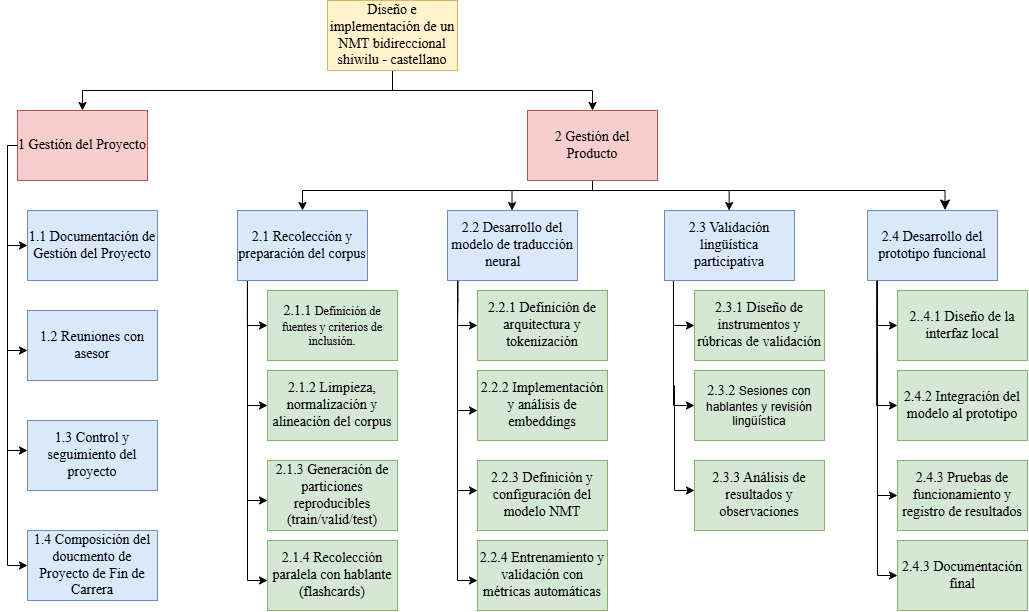
\includegraphics[width=\linewidth,alt={Diagrama de la estructura de descomposición del trabajo}]{media/image3.png}
\end{center}

La Estructura de Descomposición del Trabajo (EDT) constituye una representación jerárquica que organiza las actividades del proyecto en componentes manejables y verificables. En el caso del presente trabajo, la EDT se divide en dos secciones principales: la Gestión del Proyecto, que comprende las tareas administrativas, académicas y de seguimiento vinculadas al curso de Proyecto de Fin de Carrera 1, y la Gestión del Producto, que abarca las fases técnicas orientadas al desarrollo del sistema de traducción automática neuronal bidireccional shiwilu--castellano.

La primera sección contempla los entregables establecidos en el curso (E1, E2 y E3), las reuniones periódicas con el asesor, el control de riesgos y avances, así como la composición final del documento de tesis. Por su parte, la gestión del producto comprende la recolección y preparación del corpus bilingüe, el modelado y entrenamiento del sistema de traducción, la validación lingüística participativa con hablantes nativos y el desarrollo del prototipo funcional. De manera complementaria, se incluye la recolección paralela de \emph{flashcards} junto al señor Fidel Lomas, orientada al fortalecimiento del vocabulario y la base de datos lingüística.

El EDT permite visualizar de forma clara la relación entre los objetivos específicos, las fases técnicas y los entregables académicos del proyecto, garantizando la trazabilidad entre las actividades, el cronograma y los resultados esperados.

\subsection*{Lista de tareas}

\begin{longtable}[]{@{}
  >{\centering\arraybackslash}p{(\linewidth - 10\tabcolsep) * \real{0.0787}}
  >{\centering\arraybackslash}p{(\linewidth - 10\tabcolsep) * \real{0.2327}}
  >{\centering\arraybackslash}p{(\linewidth - 10\tabcolsep) * \real{0.1372}}
  >{\centering\arraybackslash}p{(\linewidth - 10\tabcolsep) * \real{0.1379}}
  >{\centering\arraybackslash}p{(\linewidth - 10\tabcolsep) * \real{0.1380}}
  >{\centering\arraybackslash}p{(\linewidth - 10\tabcolsep) * \real{0.2755}}@{}}
\caption{Lista de tareas (EDT)}\label{tab:edt-tareas}\\
\toprule
\textbf{EDT} & \textbf{Nombre de la tarea} & \textbf{Duración (días)} & \textbf{Esfuerzo (h-persona)} & \textbf{Costo estimado (S/.)} & \textbf{Método de verificación y validación} \\
\midrule
\endfirsthead
\caption*{\tablename~\thetable\ (continuación)}\\
\toprule
\textbf{EDT} & \textbf{Nombre de la tarea} & \textbf{Duración (días)} & \textbf{Esfuerzo (h-persona)} & \textbf{Costo estimado (S/.)} & \textbf{Método de verificación y validación} \\
\midrule
\endhead
\midrule
\endfoot
\bottomrule
\endlastfoot
1.1.1 & Avance del cronograma y envío inicial & 7 & 8 & 80 & Revisión del cronograma inicial y validación con asesor \\
1.1.2 & E1 -- Plan de Proyecto & 19 & 20 & 200 & Entrega revisada y aprobada / asesor \\
1.1.3 & E2 -- Marco conceptual y estado del arte & 27 & 28 & 280 & Retroalimentación del asesor y validación del profesor del curso \\
1.1.4 & E3 -- Plan de proyecto y correcciones finales & 36 & 32 & 320 & Revisión del asesor y calificación final del curso \\
1.2 & Reuniones con asesor de tesis & 84 & 13 & 130 & Correos de confirmación de reunión semanal \\
1.3 & Control y seguimiento del proyecto & 60 & 25 & 90 & Bitácora de avances y reportes de progreso \\
1.4 & Composición del documento de tesis & 45 & 40 & 400 & Revisión de formato PUCP y observaciones resueltas \\
2.1.1 & Definición de fuentes y criterios de inclusión & 10 & 12 & 100 & Lista validada y aprobada por asesor \\
2.1.2 & Limpieza y alineación del corpus & 20 & 28 & 6 & Comparación con corpus original y bitácora de preprocesamiento \\
2.1.3 & Generación de particiones reproducibles & 5 & 10 & 20 & Scripts reproducibles y revisión de semillas \\
2.1.4 & Recolección paralela con hablante (flashcards) & 84 & 25 & 250 & Validación lingüística con hablante (Grupo Chana / Fidel Lomas Chota) \\
2.2.1 & Definición de arquitectura y tokenización & 10 & 20 & 45 & Configuración aprobada y reproducible \\
2.2.2 & Implementación y análisis de \emph{embeddings} & 6 & 20 & 45 & Reporte técnico y comparación de resultados \\
2.2.3 & Entrenamiento y pruebas del modelo & 12 & 60 & 220 & Registro de métricas y logs de entrenamiento \\
2.2.4 & Optimización final del sistema & 5 & 25 & 50 & Evaluación de desempeño final del modelo \\
2.3.1 & Diseño de instrumentos de validación & 3 & 12 & 25 & Aprobación del instrumento por asesor \\
2.3.2 & Sesiones con hablantes y revisión lingüística & 5 & 15 & 30 & Rúbricas completadas y observaciones registradas \\
2.3.3 & Análisis de resultados y observaciones & 4 & 15 & 30 & Informe consolidado con tablas y conclusiones \\
2.4.1 & Diseño de la interfaz local & 10 & 18 & 80 & Prueba funcional en entorno local \\
2.4.2 & Integración del modelo al prototipo & 6 & 25 & 50 & Verificación de inferencias correctas \\
2.4.3 & Pruebas de funcionamiento y registro de resultados & 5 & 20 & 40 & Registro de casos de prueba y evidencias \\
2.4.4 & Documentación final y demo & 4 & 15 & 30 & Presentación y revisión del prototipo \\
\end{longtable}

\subsection*{Cronograma del proyecto}

\begin{longtable}[]{@{}
  >{\centering\arraybackslash}p{(\linewidth - 10\tabcolsep) * \real{0.0787}}
  >{\centering\arraybackslash}p{(\linewidth - 10\tabcolsep) * \real{0.2473}}
  >{\centering\arraybackslash}p{(\linewidth - 10\tabcolsep) * \real{0.1520}}
  >{\centering\arraybackslash}p{(\linewidth - 10\tabcolsep) * \real{0.1477}}
  >{\centering\arraybackslash}p{(\linewidth - 10\tabcolsep) * \real{0.1760}}
  >{\centering\arraybackslash}p{(\linewidth - 10\tabcolsep) * \real{0.1982}}@{}}
\caption{Cronograma del proyecto}\label{tab:cronograma}\\
\toprule
\textbf{EDT} & \textbf{Nombre de la tarea} & \textbf{Fecha de inicio} & \textbf{Fecha de fin} & \textbf{Duración planificada (días)} & \textbf{Dependencias} \\
\midrule
\endfirsthead
\caption*{\tablename~\thetable\ (continuación)}\\
\toprule
\textbf{EDT} & \textbf{Nombre de la tarea} & \textbf{Fecha de inicio} & \textbf{Fecha de fin} & \textbf{Duración planificada (días)} & \textbf{Dependencias} \\
\midrule
\endhead
\midrule
\endfoot
\bottomrule
\endlastfoot
1 & Gestión del proyecto & 19/08/2025 & 19/11/2025 & --- & --- \\
1.1 & Entregables del curso de Tesis 1 (PFC1) & 19/08/2025 & 19/11/2025 & --- & --- \\
& Avance del cronograma y envío inicial & 19/08/2025 & 25/08/2025 & 7 & --- \\
& E1 -- Plan de Proyecto & 27/08/2025 & 15/09/2025 & 20 & 1.1 \\
& E2 -- Marco conceptual y estado del arte & 17/09/2025 & 13/10/2025 & 27 & 1.1 \\
& E3 -- Plan de proyecto y correcciones finales & 15/10/2025 & 19/11/2025 & 36 & 1.1 \\
1.2 & Reuniones con el asesor de tesis & 23/08/2025 & 15/11/2025 & 84 & Paralelo a todas las tareas \\
1.4 & Composición y edición del documento de tesis & 19/08/2025 & 19/11/2025 & 93 & Paralelo a todo el proyecto \\
2 & Gestión del producto & 17/02/2026 & 05/07/2026 & --- & --- \\
2.1 & Recolección y preparación del corpus & 17/02/2026 & 27/03/2026 & --- & --- \\
2.1.1 & Definición de fuentes y criterios de inclusión & 17/02/2026 & 28/02/2026 & 10 & --- \\
2.1.2 & Limpieza y alineación del corpus & 02/03/2026 & 20/03/2026 & 20 & 2.1.1 \\
2.1.3 & Generación de particiones reproducibles & 23/03/2026 & 27/03/2026 & 5 & 2.1.2 \\
2.1.4 & Recolección paralela con hablante (flashcards) & 17/02/2026 & 10/05/2026 & 84 & Paralela \\
2.2 & Desarrollo del modelo de traducción & 30/03/2026 & 13/05/2026 & --- & 2.1.3 \\
2.2.1 & Definición de arquitectura y tokenización & 30/03/2026 & 10/04/2026 & 10 & 2.1.3 \\
2.2.2 & Implementación y análisis de embeddings & 13/04/2026 & 20/04/2026 & 6 & 2.2.1 \\
2.2.3 & Entrenamiento y pruebas del modelo & 21/04/2026 & 06/05/2026 & 12 & 2.2.2 \\
2.2.4 & Optimización final del sistema & 07/05/2026 & 13/05/2026 & 5 & 2.2.3 \\
2.3 & Validación lingüística participativa & 14/05/2026 & 30/05/2026 & --- & 2.2.4 \\
2.3.1 & Diseño de instrumentos de validación & 14/05/2026 & 16/05/2026 & 3 & 2.2.4 \\
2.3.2 & Sesiones con hablantes y revisión lingüística & 18/05/2026 & 24/05/2026 & 5 & 2.3.1 \\
2.3.3 & Análisis de resultados y observaciones & 25/05/2026 & 30/05/2026 & 4 & 2.3.2 \\
2.4 & Desarrollo del prototipo funcional & 01/06/2026 & 05/07/2026 & --- & 2.3.3 \\
2.4.1 & Diseño de la interfaz local & 01/06/2026 & 12/06/2026 & 10 & 2.3.3 \\
2.4.2 & Integración del modelo al prototipo & 15/06/2026 & 22/06/2026 & 6 & 2.4.1 \\
2.4.3 & Pruebas de funcionamiento y registro de resultados & 23/06/2026 & 29/06/2026 & 5 & 2.4.2 \\
2.4.4 & Documentación final y demo & 30/06/2026 & 05/07/2026 & 4 & 2.4.3 \\
\end{longtable}

\begin{itemize}
\item
  Lista de recursos

  \begin{itemize}
  \item
    Personas involucradas y necesidades de capacitación

    \begin{itemize}
    \item
      Tesista: Fabian Fernando Prado Infanson
    \item
      Asesor: Mg. Héctor Erasmo Gomez Montoya
    \item
      Colaboradores:

      \begin{itemize}
      \item
        Fidel Lomas Chota: hablante nativo shiwilu, colaborador en la elaboración de flashcards y validación participativa.
      \end{itemize}
    \item
      Necesidad de Capacitación:

      \begin{itemize}
      \item
        Las actividades a realizar el proyecto en el proyecto de fin de carrera se encuentran dentro del ámbito de la Ingeniería Informática y están respaldadas por los conocimientos adquiridas en cursos electivos de la especialización en Inteligencia Artificial. No se requiere capacitación adicional, aunque se reforzará el aprendizaje autodirigido mediante la revisión bibliográfica técnica actualizada sobre NMT.
      \end{itemize}
    \end{itemize}
  \item
    Materiales requeridos para el proyecto

    \begin{itemize}
    \item
      Electricidad
    \item
      Servicio de internet
    \item
      Acceso a bibliografía y repositorios digitales ( IEEXplore, arXiv, Github).
    \end{itemize}
  \item
    Estándares utilizados en el proyecto

    \begin{itemize}
    \item
      ISO/IEC 29110-5-1-2 -- Gestión de proyectos para Very Small Entities (VSE).
    \item
      Directrices éticas para la recolección y tratamiento de datos lingüísticos (basadas en ACL Ethics 2023).
    \item
      Normas institucionales PUCP para la elaboración de trabajos de fin de carrera.
    \item
      Principios FAIR de gestión y reutilización de datos (Findable, Accessible, Interoperable, Reusable).
    \end{itemize}
  \item
    Equipamiento requerido

    \begin{itemize}
    \item
      Computadora personal con procesador Intel i7, 32 GB RAM y GPU RTX 5060 TI 16GB.
    \end{itemize}
  \item
    Herramientas requeridas

    \begin{itemize}
    \item
      Python, PyTorch, Hugging Face Transformers y SentencePiece.
    \item
      Google Colab Pro / Kaggle como entornos de cómputo.
    \end{itemize}
  \end{itemize}
\item
  Costeo del Proyecto
\end{itemize}

\textless\textless{} Debe desarrollar un análisis de costos que incluya siempre:

\begin{itemize}
\item
  costos por el equipo humano
\item
  costos por utilización de equipamiento (usar el concepto de depreciación)
\item
  costos por utilización de software, usar el concepto de TCO (Total cost of ownership) o amortización
\item
  Debe tener claro que costo es un concepto distinto al de gasto
\end{itemize}

A continuación, se presenta una plantilla mínima genérica que puede ser usada de base para establecer un presupuesto. Para los proyectos de curso es suficiente un solo nivel de partida.

\begin{longtable}[]{@{}
  >{\raggedright\arraybackslash}p{(\linewidth - 12\tabcolsep) * \real{0.0692}}
  >{\raggedright\arraybackslash}p{(\linewidth - 12\tabcolsep) * \real{0.1778}}
  >{\centering\arraybackslash}p{(\linewidth - 12\tabcolsep) * \real{0.1307}}
  >{\centering\arraybackslash}p{(\linewidth - 12\tabcolsep) * \real{0.1327}}
  >{\centering\arraybackslash}p{(\linewidth - 12\tabcolsep) * \real{0.1303}}
  >{\centering\arraybackslash}p{(\linewidth - 12\tabcolsep) * \real{0.1565}}
  >{\centering\arraybackslash}p{(\linewidth - 12\tabcolsep) * \real{0.1308}}@{}}
\caption{Presupuesto del proyecto}\label{tab:presupuesto}\\
\toprule
\textbf{Ítem} & \textbf{Descripción} & \textbf{Unidad} & \textbf{Cantidad} & \textbf{Valor unidad (S/.)} & \textbf{Monto parcial (S/.)} & \textbf{Monto total (S/.)} \\
\midrule
\endfirsthead
\caption*{\tablename~\thetable\ (continuación)}\\
\toprule
\textbf{Ítem} & \textbf{Descripción} & \textbf{Unidad} & \textbf{Cantidad} & \textbf{Valor unidad (S/.)} & \textbf{Monto parcial (S/.)} & \textbf{Monto total (S/.)} \\
\midrule
\endhead
\midrule
\endfoot
\bottomrule
\endlastfoot
\textbf{0} & \textbf{Costo total del proyecto} & - & - & - & - & \textbf{13665.00} \\
\textbf{1} & \textbf{Tesista} & - & - & - & - & \textbf{4600.00} \\
1.1 & Fabian Prado Infanson & Hora & 460 & 10 & 4600 & - \\
\textbf{2} & \textbf{Otros participantes} & - & - & - & - & \textbf{2240.00} \\
2.1 & Mg. H. Erasmo Gómez Montoya (Asesor académico) & Hora & 37 & 20 & 740 & - \\
2.2 & Fidel Lomas Chota & Hora & 100 & 15 & 1500 & - \\
\textbf{3} & \textbf{Materiales e insumos} & - & - & - & - & \textbf{1625.00} \\
3.1 & Electricidad & Mes & 9 & 25 & 225 & - \\
3.2 & Servicio de internet & Mes & 9 & 100 & 900 & - \\
3.3 & Google Colab Pro & Mes & 5 & 100 & 500 & \\
\textbf{4} & \textbf{Equipamiento y software} & - & - & - & - & \textbf{5200.00} \\
4.1 & Computadora personal & Unidad & 1 & 5000 & 5000 & - \\
4.2 & Microsoft Office Suite & Anual & 1 & 200 & 200 & - \\
\end{longtable}

\end{document}
